\chapter{定理证明与模型检测的结合}\label{chapt:sctl}
本章首先介绍逻辑系统\CTLP{},\CTLP{}是计算树逻辑\CTL{}的一个扩展;然后介绍针对\CTLP{}的一个证明系统\SCTL{}; 最后介绍针对证明系统\SCTL{}的一个证明搜索策略及其伪代码。

\section{\CTLP{}}\label{sec:ctlp}
我们用逻辑 \CTLP{($\cal M$)} 来刻画要验证的系统 $\cal M$ 的性质,其中 $\cal M$ 通常指的是一个 Kripke 结构,其定义如下。
\begin{definition}[Kripke 结构]
	一个 Kripke 结构 $\cal M = (S, \lra, \mathcal{P})$ 包含如下三个部分:
	\begin{enumerate}
		\item $S$ 是一个有穷的状态集合;
		\item $\lra\;\subseteq S \times S$ 是一个一个二元关系 ;对于每一个状态 $s\in S$,至少存在一个 $s'\in S$ 使得 $s\lra s'$;
		\item $\mathcal{P}$ 是一个有穷的关系符号的集合;对于每个关系符号 $P\in \mathcal{P}$,都存在自然数 $n$ 使得$P\in S^n$ 。
	\end{enumerate}
\end{definition}
对于一个状态 $s\in S$,我们将 $s$ 的所有的下一个状态的集合定义为
\begin{center}
	$\nextstate{s} = \{s'\mid s\lra s'\}$。 
\end{center} 
一个路径是一个有穷或无穷的状态序列,通常形式为 $s_0,...,s_n$ 或者 $s_0,s_1,...$ ,其中,对于任意自然数$i$,如果 $s_i$ 不是该序列的最后一个元素,那么就有 $s_{i+1}\in \nextstate{s_i}$ 。

我们称 $T$ 是一棵\textit{路径树}当且仅当对于 $T$ 上的所有由 $s$ 标记的非叶子节点,该节点的所有后继节点正好由 $\nextstate{s}$ 中的所有元素一一标记。一棵路径树上的所有节点既可以是有穷个也可以是无穷个。


\paragraph{语法。}一个Kripke 结构 $\cal M$ 的性质由 \CTLP{}$(\cal M)$ 公式表示:
\begin{definition}\label{def:ctlp}
    对于一个给定的Kripke模型 $\cal M = (S, \lra, \mathcal{P})$,\CTLP{}$(\cal M)$公式的语法定义如下:
%    \begin{center}
        $$\phi \ :=
        \left\{\begin{array}{l}
        \top\ | \ \bot \ | \ P(t_1, ..., t_n)\  | \neg P(t_1, ..., t_n)\  | \ \phi  \wedge \phi \ |\ \phi \vee \phi \ | \\
        \ AX_x(\phi)(t)\ | \ EX_x(\phi)(t) \ | \ AF_x(\phi)(t) \ | \ EG_x(\phi)(t) \ |\\
        \ AR_{x,y}(\phi_1,\phi_2)(t)\ | \ EU_{x,y}(\phi_1,\phi_2)(t)
        \end{array}
        \right.$$
%    \end{center}
    其中,$x$ 与 $y$ 为变量,取值范围为 $S$,而 $t_1,...,t_n$ 既可以是代表状态的常量,也可以是取值范围为 $S$ 的变量。
\end{definition}
在定义~\ref{def:ctlp} 中,我们用模态词来绑定公式中的变量。比如,模态词 $AX$,$EX$, $AF$ 以及 $EG$ 在公式 $\phi$ 中绑定了变量 $x$;而模态词 $AR$ 和 $EU$ 则在公式 $\phi_1$ 和 $\phi_2$ 中分别绑定了变量 $x$ 和 $y$. 变量的替换则写为 $(t/x)\phi$,表示将公式 $\phi$ 中所有自由出现的变量 $x$ 都替换为 $t$。

不失一般性地来说,我们假定所有的否定符号都出现在原子命题上;而且有如下缩写:
\begin{itemize}
	\item $\phi_1\A \phi_2 \equiv \neg \phi_1 \vee \phi_2$,
	\item $EF_x(\phi)(t) \equiv EU_{z,x}(\top, \phi)(t)$,
	\item $ER_{x, y}(\phi_1,\phi_2)(t) \equiv EU_{y,z}(\phi_2,((z/x)\phi_1 \wedge
	(z/y)\phi_2))(t)\vee EG_y(\phi_2)(t)$, 其中变量 $z$ 既不在 $\phi_1$,也不在 $\phi_2$ 中出现,
	\item $AG_x(\phi)(t) \equiv \neg (EF_x(\neg \phi)(t))$,
	\item $AU_{x,y}(\phi_1,\phi_2)(t) \equiv \neg (ER_{x,y}(\neg\phi_1,\neg\phi_2)(t))$.
\end{itemize}
我们称模态词 $AF$,$EF$,$AU$,以及 $EU$ 为\textit{归纳模态词};
模态词 $AR$,$ER$,$AG$,以及 $EG$ 为\textit{余归纳模态词}。

\paragraph{语义。}相应地,对于一个给定的 Kripke 模型 $\cal M$,\CTLP{($\cal M$)}的语义定义如下:
\begin{itemize}
	\item ${\cal M}\models P(s_1,...,s_n)$:如果$\langle s_1,...,s_n\rangle\in P$,而且$P$是一个$\cal M$上的$n$元关系;
	\item ${\cal M}\models \neg P(s_1,...,s_n)$:如果$\langle s_1,...,s_n\rangle\notin P$,而且$P$是一个$\cal M$上的$n$元关系;
	\item ${\cal M}\models \top$ 永远成立;
	\item ${\cal M}\models \bot$ 永远不成立;
	\item ${\cal M}\models \phi_1\wedge\phi_2$:如果${\cal M}\models \phi_1$和 ${\cal M}\models \phi_2$同时成立;
	\item ${\cal M}\models \phi_1\vee\phi_2$:如果${\cal M}\models \phi_1$成立,或者 ${\cal M}\models \phi_2$成立;
	\item ${\cal M}\models AX_x(\phi_1)(s)$:如果对于每个状态$s'\in\textsf{Next}(s)$,都有${\cal M}\models (s'/x)\phi_1$成立;
	\item ${\cal M}\models EX_x(\phi_1)(s)$:如果存在一个状态$s'\in\textsf{Next}(s)$,使得${\cal M}\models (s'/x)\phi_1$成立;
	\item ${\cal M}\models AF_x(\phi_1)(s)$:如果存在一个有无穷个节点的树$T$,而且 $T$的根节点是$s$,那么对于$T$的任何一个非叶子节点$s'$,$s'$的子节点为\nextstate{$s'$},对于$T$的任何一个叶子节点$s'$,$\vdash (s'/x)\phi_1$成立;
	\item ${\cal M}\models EG_x(\phi_1)(s)$:如果存在$\cal M$上的一个无穷路径 $s_0,s_1,...$(其中 $s_0 = s$),那么对于任意的自然数 $i$,都有 ${\cal M}\models (s_i/x)\phi_1$成立;
	\item ${\cal M}\models AR_{x, y}(\phi_1,\phi_2)(s)$:如果存在一棵路径树 $T$,$T$ 的根节点由 $s$ 标记,对于任意节点 $s'\in T$ 都有 $\mathcal{M}\models (s'/y)\phi_2$ 成立,而且对于任意的叶子节点 $s''\in T$ 都有 $\mathcal{M}\models (s''/x)\phi_1$ 成立;
	\item ${\cal M}\models EU_{x, y}(\phi_1,\phi_2)(s)$:如果存在一个无穷路径 $s_0,s_1,...$(其中 $s_0=s$)和一个自然数 $j$,$\mathcal{M}\models(s_j/y)\phi_2$ 成立,而且对于任意的自然数 $i<j$ 都有 $\mathcal{M}\models (s_i/x)\phi_1$ 成立。
\end{itemize}


\paragraph{\CTL{} vs. \CTLP{}。}在计算树逻辑(\CTL)\cite{EmersonC82,EmersonH85} 的语法中,原子公式通常用命题符号来表示,而命题符号在计算树逻辑的语义中通常解释为一个 Kripke 结构上的状态集合。在逻辑系统\CTLP{}中,相比于计算树逻辑,我们通过引入多元谓词来增加逻辑系统中公式的表达能力。\CTLP{}相比于\CTL{}的表达能力的提升可由如下的例子表示出来:

\begin{example}\label{example:unmanned}
	本例子受多机器人路径规划系统\cite{Craig89,PartoviL14}启发。在原例子中,多机器人路径规划系统的规范可以写成 \CTL{} 公式:在一个多个区块的地图上,每从初始位置出发的机器人都能到达指定的最终位置,而且在行进的同时,每个机器人都会避免经过某些位置。
	
	在本例子中,除了\CTL{}所能表示的时序性质之外,我们考虑一种“空间”性质,即表示状态之间的关系。
	
	假定有一个无人车正在一个星球表面行驶,这个星球的表面已经被分成了有穷个小的区域。无人车一次能从一个区域行走到另一个区域,那么我们将无人车的位置看作成一个状态,无人车所有的可能的所在位置则可看作为状态空间,而且无人车从一个位置到另一个位置的移动规律则可看作成迁移关系。无人车的设计需要满足一个基本的性质,即无人车不能永远在一个很小的范围内移动。准确地说,对于给定的距离 $\sigma$,在任意状态 $s$,随着无人车的移动会到达状态 $s'$,使得 $s$ 和 $s'$ 的位置之间的距离大于 $\sigma$。该性质可以由公式 $AG_x(AF_y(D_\sigma(x,y))(x))(s_0)$ 来刻画,其中 $s_0$ 是初始状态,即无人车的降落点;原子公式 $D_\sigma(x,y)$ 则刻画了一种空间性质,即状态 $x$ 和 $y$ 的位置的距离大于 $\sigma$。
	
	\begin{figure}[h]
		\centering
		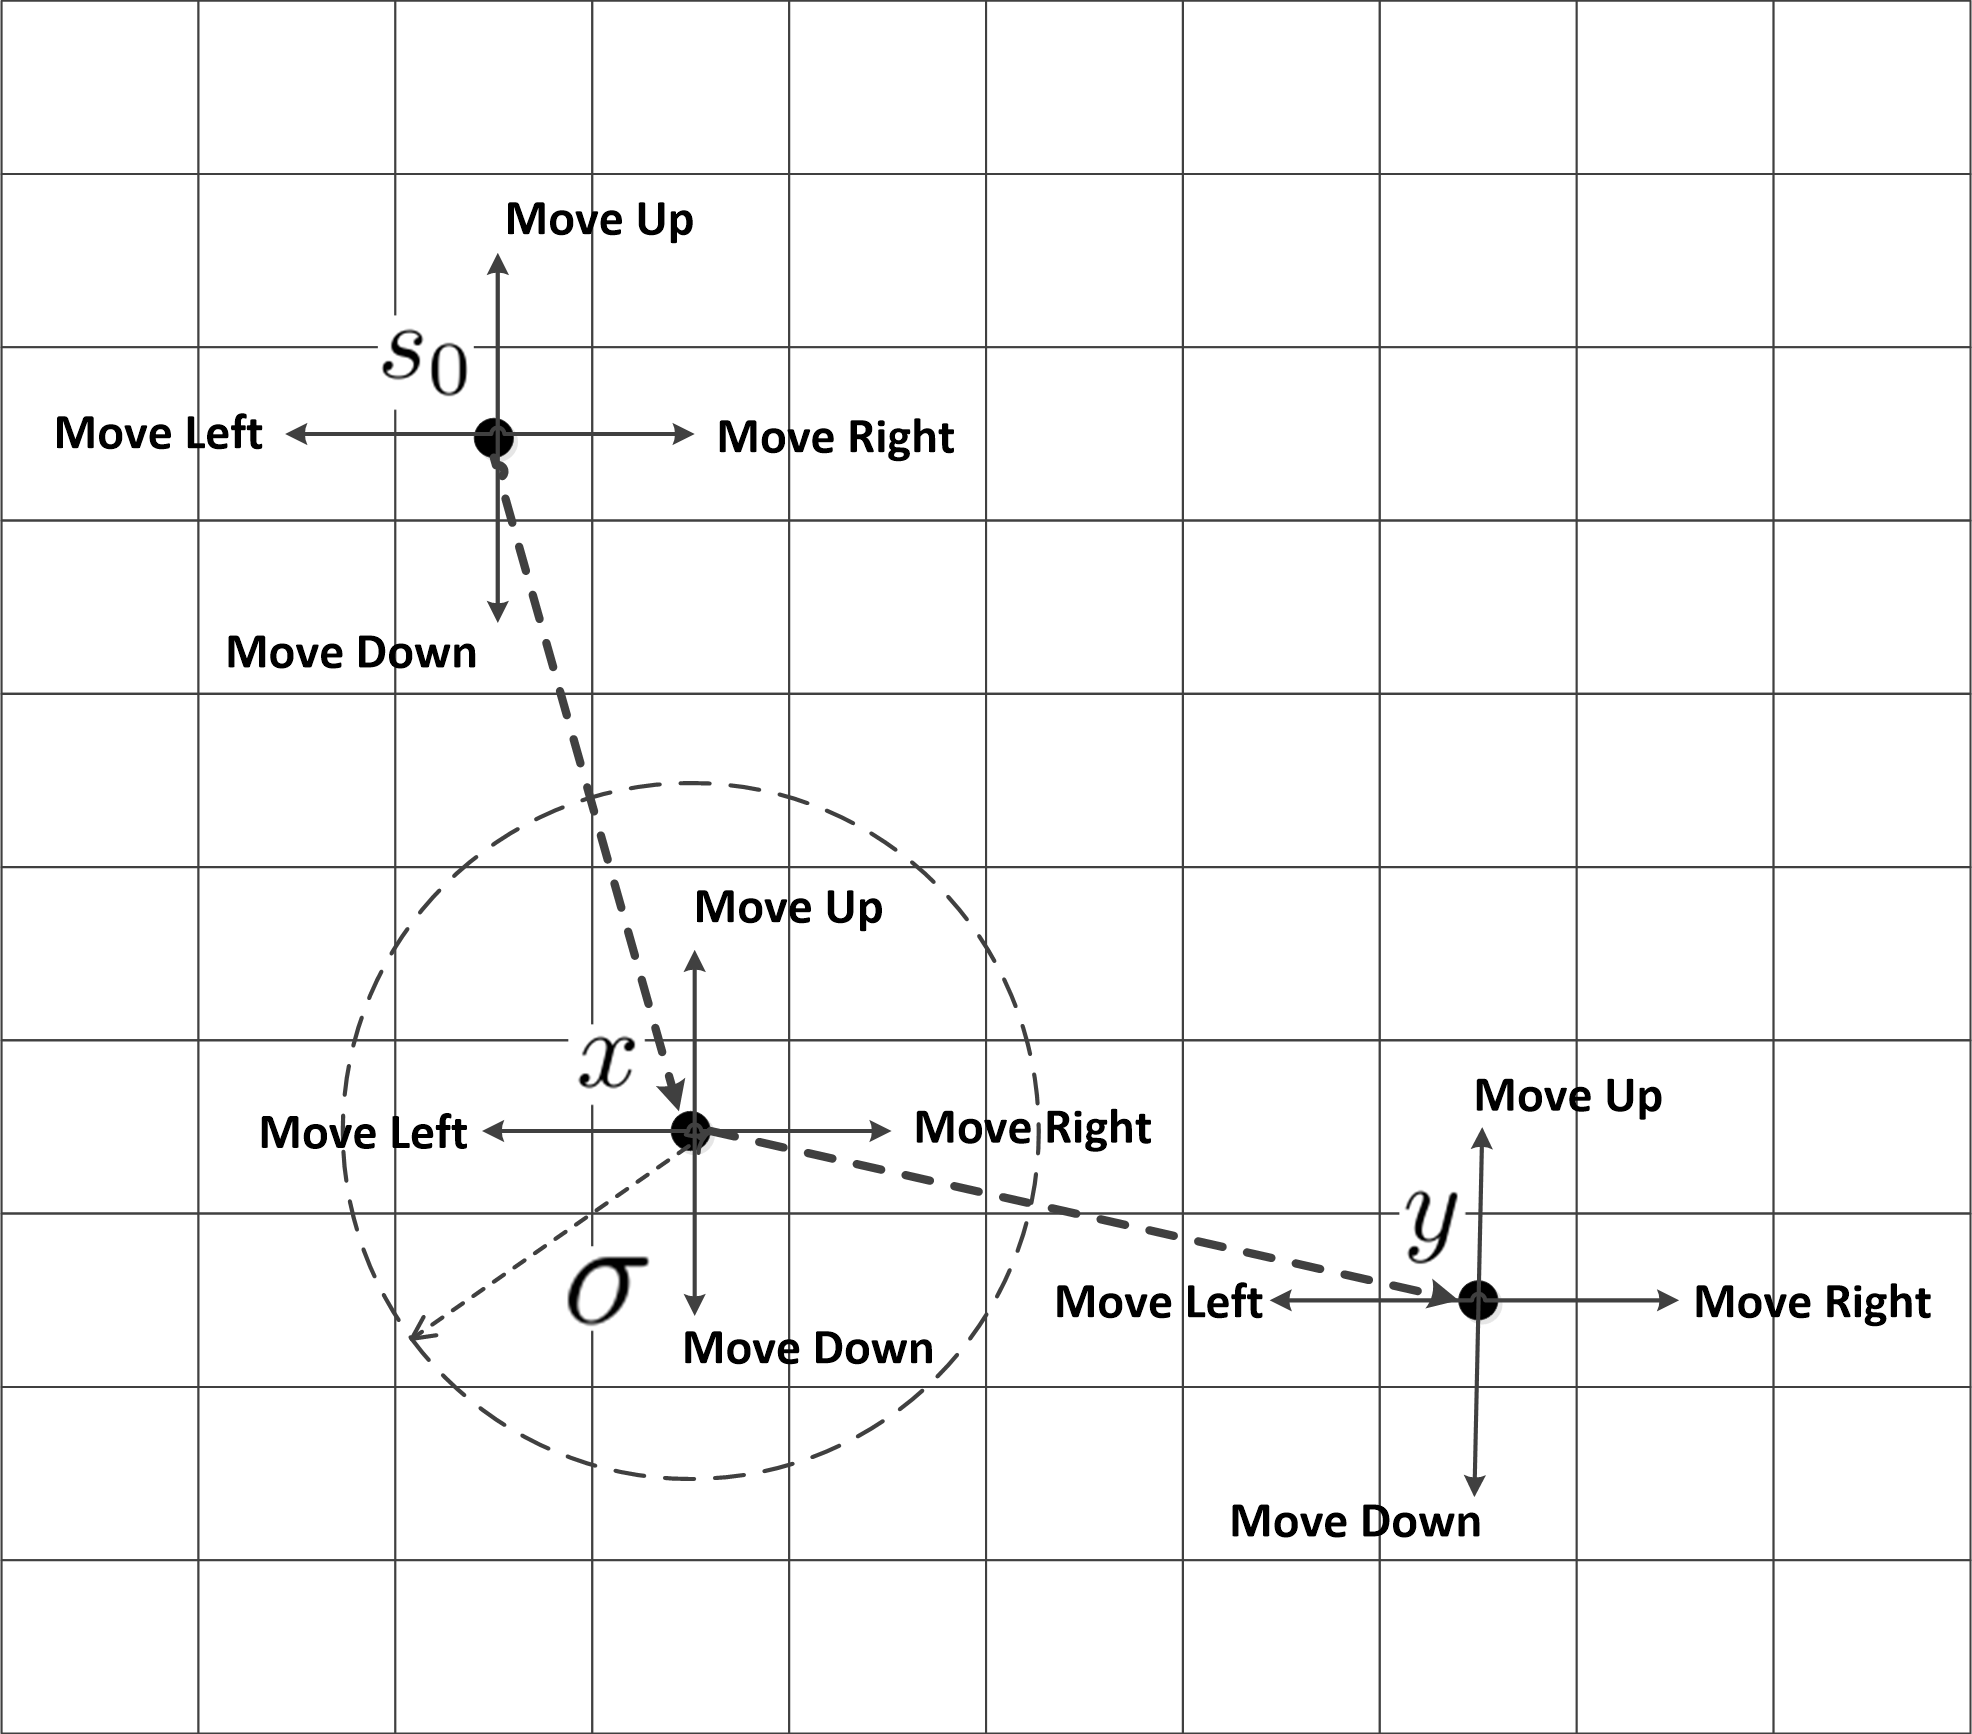
\includegraphics[width=10cm]{uv}
		\caption{无人车可能的所在位置}\label{fig:uv}
	\end{figure}
	
\end{example}

例子\ref{example:unmanned}中的性质可以很容易由 \CTLP{} 中的公式进行刻画,然而很难用传统的时序逻辑的公式进行表示。原因是在传统的时序逻辑的语法中通常没有表述一个特定的状态或者多个状态之间的关系的机制,即使在语义中,传统的时序逻辑通常只考虑当前的状态,而无法考虑多个状态之间的关系。

\section{\CTLP{}的证明系统:\SCTL{}}\label{sec:sctl}
在本节,我们针对逻辑 \CTLP$(\cal M)$ 给出一个证明系统 \sctlm{} (Sequent-calculus-like proof system for \CTLP{})。在通常意义下的证明系统中,一个公式是可证的当且仅当该公式在所有的模型中都成立,而在 \sctlm{} 中,一个公式是可证的当且仅当该公式在模型 $\cal M$ 中是可证的。

首先,让我们考虑一个\ctlpm{}公式 $AF_x(P(x))(s)$。该公式在模型 $\cal M$ 中成立当且仅当存在一个路径树 $T$,$T$ 的根节点由 $s$ 标记,而且 $T$ 上的每个叶子节点都满足 $P$。\couic{这样的路径树 $T$ 可被用来验证公式 $AF_x(P(x))(s)$ 的成立。}

然后,我们考虑一个具有嵌套模态词的 \CTLP$(\cal M)$ 公式 $AF_x(AF_y(P(x,y))(x))(s)$。如果试图说明该公式在模型 $\cal M$ 中是成立的,那么就需要找到一个路径树 $T$,使得 $T$ 的根节点由 $s$ 标记,而且对于 $T$ 中的所有叶子节点 $a$,$AF_y(P(a,y))(a)$ 是成立的。为了说明 $AF_y(P(a,y))(a)$ 是成立的,则需要又找到一棵路径树 $T'$ 使得 $T'$ 的根节点由 $a$ 标记,而且 $T'$ 上的所有叶子节点 $b$ 都满足 $P(a,b)$。我们可以用以下的两个规则来刻画当前的嵌套的路径树。
\begin{center}
	$\infer[^{\mbox{\small $\mathbf{AF}$-{$\mathsf{R_1}$}}}]{\vdash AF_x(\phi)(s)}{\vdash (s/x)\phi}$\\
	\vspace{10pt}
	$\infer[^{\mbox{\small $\mathbf{AF}$-{$\mathsf{R_2}$}}}_{\{s_1,...s_n\}=\textsf{Next}(s)}]{\vdash AF_x(\phi)(s)}
	{\vdash AF_x(\phi)(s_1) & \ldots & \vdash AF_x(\phi)(s_n)}$
\end{center}

\begin{example}\label{example:exp2}
	假设一个模型有如下图所示的迁移规则,
		\begin{center}
			\centering
			\begin{tikzpicture}
			[scale=1.5,->,>=stealth',shorten >=1pt,auto,inner sep=2pt,semithick,bend angle=20]
			\tikzstyle{every state}=[draw=none] 
			\node[state] (1) at (0,0) {$a$};
			\node[state] (2) at (1,0.3) {$b$}; 
			\node[state] (3) at (1,-0.3){$c$}; 
			\node[state] (4) at (2,0) {$d$};
			
			\draw[right] (0.1,0.05) -- (0.9,0.25);
			\draw[right] (0.1,-0.05) -- (0.9,-0.25);
			\draw[right] (1.1,0.25) -- (1.9,0.05);
			\draw[right] (1.1,-0.25) -- (1.9,-0.05);
			\draw[->] (2.1,0.1) arc (-20:-325:-0.2);
			\end{tikzpicture}
		\end{center}
		和一个原子谓词 $P=\{b, c\}$,那么公式 $AF_x(P(x))(a)$ 的一个证明如下。
		$$\infer[{\mbox{\small $\mathbf{AF}$-{$\mathsf{R_2}$}}}]{\vdash
			AF_x(P(x))(a)}{\infer[\mbox{\small $\mathbf{AF}$-{$\mathsf{R_1}$}}]{\vdash
				AF_x(P(x))(b)}{\infer[\mbox{\small atom-\textsf{R}}]{\vdash P(b)}{}} \quad\quad
			\infer[\mbox{$\mathbf{AF}$-{$\mathsf{R_1}$}}]{\vdash
				AF_x(P(x))(c)}{\infer[\mbox{\small atom-\textsf{R}}]{\vdash P(c)}{}}}$$
		在此证明树中,除了 $\mathbf{AF}$-{$\mathsf{R_1}$} 和 $\mathbf{AF}$-{$\mathsf{R_2}$},我们还应用了如下规则。 
		\begin{center}
			$\infer[^{\mbox{atom-\textsf{R}}}_{\langle s_1,...,s_n\rangle\in P}]{\vdash P(s_1,...,s_n)}{}$
		\end{center}
\end{example}


\begin{example}\label{example:exp3}
		假设另一个模型,该模型的迁移规则与例子\ref{example:exp2}中相同,除此之外还有原子谓词 $Q=\{(b,d), (c,d)\}$。
		公式 $AF_x(AF_y(Q(x, y))(x))(a)$ 的证明如下。
		
		$$\infer[{\mbox{\small $\mathbf{AF}$-{$\mathsf{R_2}$}}}]
		{\vdash AF_x(AF_y(Q(x, y))(x))(a)}
		{\infer[\mbox{$\mathbf{AF}$-{$\mathsf{R_1}$}}]
			{\vdash AF_x(AF_y(Q(x, y))(x))(b)}
			{\infer[{\mbox{\small $\mathbf{AF}$-{$\mathsf{R_2}$}}}]
				{\vdash AF_y(Q(b, y))(b)}
				{\infer[\mbox{\small $\mathbf{AF}$-{$\mathsf{R_1}$}}]
					{\vdash AF_y(Q(b, y))(d)}
					{\infer[\mbox{\small atom-\textsf{R}}]
						{Q(b,d)}
						{}
					}
				}
			}
			\quad\quad
			\infer[\mbox{$\mathbf{AF}$-{$\mathsf{R_1}$}}]
			{\vdash AF_x(AF_y(Q(x, y))(x))(b)}
			{\infer[{\mbox{\small $\mathbf{AF}$-{$\mathsf{R_2}$}}}]
				{\vdash AF_y(Q(c, y))(c)}
				{\infer[\mbox{\small $\mathbf{AF}$-{$\mathsf{R_1}$}}]
					{\vdash AF_y(Q(c, y))(d)}
					{\infer[\mbox{\small atom-\textsf{R}}]
						{Q(c,d)}
						{}
					}
				}
			}
		}$$
		
\end{example}


\couic{
	Note that \SCTL{} needs neither contraction rules nor multiplicative
$\vee$-\textsf{R} rules, because for each atomic formula $P$, either
$P$ is provable or $\neg P$ is.  Therefore the sequent $\vdash \neg P
\vee P$ is proved by proving either the sequent $\vdash \neg P$ or the
sequent $\vdash P$. 
As we have neither multiplicative $\vee$-\textsf{R} rules nor
structural rules, if we start with a sequent $\vdash \phi$ where the formula $\phi$ does not have co-inductive sub-formulae, then each
sequent in the proof has one formula on the right of $\vdash$ and none
on the left.
}
在\SCTL{}中,每个相继式都有$\Gamma\vdash\phi$形式,其中$\Gamma$是一个可能为空的\SCTL{}公式集合,$\phi$是一个\SCTL{}公式。 不同于通常的相继式演算,
%如果 $P$ 是一个原子公式,那么 $P$ 是可证的或者 $\neg P$ 是可证的。

So, as all sequents have the form $\vdash \phi$, the left rules and
the axiom rule can be dropped as well.  In other words, unlike the
usual sequent calculus and like Hilbert systems, \SCTL{} is tailored for
deduction, not for hypothetical deduction.



As the left-hand side of sequents is not used to record hypotheses, 
we will use it to record a different kind of information, that occur
in the case of co-inductive modalities, such as the modality $EG$. 

Indeed, the case of the co-inductive formula, for example $EG_x(P(x))(s)$, is
more complex than that of the inductive one, such as $AF_x(P(x))(s)$.
To justify its validity, one needs to provide an infinite sequence starting from $s$, and each state in the infinite sequence
verifies $P$. However, as the model is finite, we can always restrict to
regular sequences and use a finite representation of such sequences. This
leads us to introduce a rule, called
$\mathbf{EG}$-\textsf{merge}, that permits to prove a sequent
of the form $\vdash EG_x(P(x))(s)$, provided such a sequent already
occurs lower in the proof. To make this rule local, we re-introduce
hypotheses $\Gamma$ to record part of the history of the proof. The
sequent have therefore the form $\Gamma\vdash\phi$, with a non empty
$\Gamma$ in this particular case only, and the
$\mathbf{EG}$-\textsf{merge} rule is then just an instance of
the axiom rule, that must be re-introduced in this particular case
only.


\SCTL{$(\cal M)$} 的证明规则如图\ref{sctl_rules}所示。

\begin{figure}[h!]
	\small
	\centering
	\noindent\framebox{\parbox{.98\textwidth}{\hspace*{-0.3cm}
			$$
			\infer[^{\mbox{atom-\textsf{R}}}_{\langle s_1,...,s_n\rangle \in P}]{\vdash P(s_1,...,s_n)}{}
			\quad \quad
			\infer[^{\mbox{$\neg$-\textsf{R}}}_{\langle s_1,...,s_n\rangle \notin P}]{\vdash \neg P(s_1,...,s_n)}{}
			$$
			\smallskip
			$$
			\infer[^{\mbox{$\top$-\textsf{R}}}]{\vdash \top}{}
			\quad\quad
			\infer[^{\mbox{$\wedge$-\textsf{R}}}]{\vdash \phi_1\wedge\phi_2}{\vdash \phi_1 & \vdash \phi_2}
			\quad\quad
			\infer[^{\mbox{$\vee$-{$\mathsf{R_1}$}}}]{\vdash \phi_1\vee\phi_2}{\vdash \phi_1}
			\quad\quad
			\infer[^{\mbox{$\vee$-{$\mathsf{R_2}$}}}]{\vdash \phi_1\vee\phi_2}{\vdash \phi_2}
			$$
			\smallskip
			$$
			\infer[^{\mbox{$\mathbf{EX}$-\textsf{R}}}_{s'\in \textsf{Next}(s)}]{\vdash EX_x(\phi)(s)}{\vdash (s'/x)\phi}
			\quad\quad
			\infer[^{\mbox{$\mathbf{AX}$-\textsf{R}}}_{\{s_1,...,s_n\}=\textsf{Next}(s)}]{\vdash AX_x(\phi)(s)}{\vdash (s_1/x)\phi & \ldots & \vdash (s_n/x)\phi}
			$$
			\smallskip
			$$
			\infer[^{\mbox{$\mathbf{AF}$-{$\mathsf{R_1}$}}}]{ \vdash AF_x(\phi)(s)}{\vdash (s/x)\phi}\quad\quad
			%$$
			%$$
			\infer[^{\mbox{$\mathbf{AF}$-{$\mathsf{R_2}$}}}_{\{s_1,...,s_n\}=\textsf{Next}(s)}]{ \vdash AF_x(\phi)(s)}{\vdash AF_x(\phi)(s_1) & \ldots & \vdash AF_x(\phi)(s_n)}
			$$
			\smallskip
			$$
			\infer[^{\mbox{$\mathbf{EG}$-\textsf{R}}}_{s' \in \textsf{Next}(s)}]{\Gamma \vdash EG_x(\phi)(s)}{\vdash (s/x)\phi & \Gamma,EG_x(\phi)(s)\vdash EG_x(\phi)(s')}\quad\quad
			%$$
			%$$
			\infer[^{\mbox{$\mathbf{EG}$-\textsf{merge}}}_{EG_x(\phi)(s)\in \Gamma}]{\Gamma \vdash EG_x(\phi)(s)}{}
			$$
			\smallskip
			$$
			\infer[^{\mbox{$\mathbf{AR}$-{$\mathsf{R_1}$}}}_{\{s_1,...,s_n\}=\textsf{{Next}}(s),\Gamma' = \Gamma,AR_{x,y}(\phi_1,\phi_2)(s)}]{\Gamma \vdash AR_{x,y}(\phi_1,\phi_2)(s)}{\vdash (s/y)\phi_2 & \Gamma'\vdash AR_{x, y}(\phi_1,\phi_2)(s_1) ~...~ \Gamma'\vdash AR_{x, y}(\phi_1,\phi_2)(s_n)}
			$$
			\smallskip
			
			
			$$
			\infer[^{\mbox{$\mathbf{AR}$-{$\mathsf{R_2}$}}}]{\Gamma \vdash AR_{x,y}(\phi_1,\phi_2)(s)}{\vdash (s/x)\phi_1 & \vdash (s/y)\phi_2}
			\quad\quad
			\infer[^{\mbox{$\mathbf{AR}$-\textsf{merge}}}_{AR_{x,y}(\phi_1,\phi_2)(s)\in \Gamma}]{\Gamma \vdash AR_{x,y}(\phi_1,\phi_2)(s)}{}
			$$
			\smallskip
			$$
			\infer[^{\mbox{$\mathbf{EU}$-{$\mathsf{R_1}$}}}]{\vdash EU_{x,y}(\phi_1,\phi_2)(s)}{\vdash (s/y)\phi_2} 
			\quad\quad
			\infer[^{\mbox{$\mathbf{EU}$-{$\mathsf{R_2}$}}}_{s'\in \textsf{Next}(s)}]{\vdash EU_{x,y}(\phi_1,\phi_2)(s)}{\vdash (s/x)\phi_1 & \vdash EU_{x,y}(\phi_1,\phi_2)(s')}
			$$
			
			
	}}
	\caption{\label{sctl_rules} \sctlm{}}
\end{figure}
\paragraph{可靠性与完备性。}\label{sound:complete}
%\SCTL{}证明系统的可靠性与完备性是基于kripke模型的有穷性。具体证明如下:
命题\ref{prop:fis}和命题\ref{prop:fit}的作用是将有穷结构转换为无穷结构,这两个命题被用来证明\SCTL{}的可靠性;命题\ref{prop:ifs}和命题\ref{prop:ift}的作用是将无穷结构转换到有穷结构,这两个命题被用来证明\SCTL{}的完备性。

\begin{proposition} [有穷状态序列到无穷状态序列]\label{prop:fis}
	给定一个有穷的状态序列$s_0,...,s_n$,其中对于任意$0\le i\le n-1$都有$s_i\longrightarrow s_{i+1}$,而且存在$0\le p \le n-1$使得$s_n=s_p$。那么,一定存在一个无穷的状态序列$s_0',s_1',...$使得$s_0 = s_0'$,而且对于任意$i\ge 0$都有$s_i'\longrightarrow
	s_{i+1}'$,同时此无穷状态序列中的每个状态都在$s_0,...,s_n$中。
\end{proposition}
\begin{proof}
	本命题所述无穷序列为:$s_0,...,s_{p-1},s_p,...,s_{n-1},s_p,...$, 其中 $s_0 = s_0'$.
\end{proof}

\begin{proposition}[有穷路径树到无穷路径树]\label{prop:fit}
	设$\Phi$为一个状态集合,$T$为一个有穷的路径树,$T$的每个叶子节点都由某个状态$s$来标记,其中,$s\in \Phi$;或者存在从$T$的根结点到当前叶子节点的分支上的一个节点,使得该节点同样由$s$所标记。那么,一定存在一棵可能无穷的路径树$T'$,而且$T'$的所有叶子节点都由$\Phi$中的某个状态标记,同时用来标记$T'$节点的状态都用来标记$T$的节点。
\end{proposition}
\begin{proof}
	令$T'$的根结点为$T$的根结点,而且对于$T$的每个节点的标记$s$来说,如果$s\in\Phi$,那么$s$标记$T'$的叶子节点;否则,$s$的后继节点分别由$\mathsf{Next}(s)$中的每个元素标记。显然,标记$T'$中节点的状态都标记$T$中的节点。
\end{proof}


\begin{proposition} [无穷状态序列到有穷状态序列]\label{prop:ifs}
	给定一个无穷状态序列$s_0,s_1,...$,其中对于任意$i\ge 0$都有$s_i\longrightarrow s_{i+1}$。那么,一定存在一个有穷的状态序列$s_0',...,s_n'$,对于任意$0\le i\le n-1$,都存在一个$0\le p\le n-1$, 使得$s_n'=s_p'$,而且$s_0',...,s_n'$中的所有状态都在$s_0,s_1,...$中出现。
\end{proposition}
\begin{proof}
	由于Kripke模型的状态集是有穷的,因此在状态序列$s_0,s_1,...$一定存在$p, n\ge 0$,使得$s_p=s_n$。本命题所述有穷状态序列即为$s_0,...,s_n$。
\end{proof}

\begin{proposition}[可能无穷的路径树到有穷路径树]\label{prop:ift}
	设$\Phi$为一个状态集合;$T$为一个可能无穷的路径树,其中$T$的所有叶子节点都由$\Phi$中的某个状态所标记。那么,一定存在一个有穷的路径树$T'$,使得对于$T'$的每个叶子节点的标记$s$,$s\in\Phi$,或者存在从$T'$的根结点到该叶子节点的分支上的一个节点,该节点同样由$s$标记。
\end{proposition}
\begin{proof}
	由于Kripke模型的状态集是有穷的,因此对于$T$的每个无穷分支,都存在$0\le p<n$,使得$s_p=s_n$。将$T$的每个这样的无穷分支在$s_n$处截断,所得到的路径树即为$T'$。显然,由于$T'$具有有穷个分支,同时$T'$的每个分支都是有穷的,因此$T'$也是有穷的。
\end{proof}

\begin{theorem}[可靠性]\label{thm:sound}
	设$\cal M$为一个Kripke模型,$\phi$为一个\ctlpm{}闭公式。如果相继式$\vdash\phi$具有一个证明,则$\mathcal{M}\models\phi$成立。
\end{theorem}
\begin{proof}
	假设相继式$\vdash\phi$具有证明$\pi$,以下对证明$\pi$的结构做归纳:
	\begin{itemize}
		\item 如果$\pi$的最后一条规则为\textsf{atom-R},那么$\vdash\phi$具有$\vdash P(s_1,...,s_n)$形式,因此$\mathcal{M}\models P(s_1,...,s_n)$。
		\item 如果$\pi$的最后一条规则为$\neg$-\textsf{R},那么$\vdash\phi$具有$\vdash \neg P(s_1,...,s_n)$形式,因此$\mathcal{M}\models \neg P(s_1,...,s_n)$。
		\item 如果$\pi$的最后一条规则为$\top$-\textsf{R},那么$\vdash\phi$具有$\vdash \top$形式,因此$\mathcal{M}\models \top$。
		\item 如果$\pi$的最后一条规则为$\wedge$-\textsf{R},那么$\vdash\phi$具有$\vdash \phi_1\wedge\phi_2$形式。根据归纳假设,$\mathcal{M}\models \phi_1$与$\mathcal{M}\models \phi_2$均成立,因此$\mathcal{M}\models \phi_1\wedge\phi_2$。
		\item 如果$\pi$的最后一条规则为$\vee$-\textsf{R},那么$\vdash\phi$具有$\vdash \phi_1\vee\phi_2$形式。根据归纳假设,$\mathcal{M}\models \phi_1$成立或$\mathcal{M}\models \phi_2$成立,因此$\mathcal{M}\models \phi_1\vee\phi_2$。
		
		\item 如果$\pi$的最后一条规则为$AX$-\textsf{R},那么$\vdash\phi$具有$\vdash AX_x(\phi_1)(s)$形式。根据归纳假设,对于任意$s'\in\mathsf{Next}(s)$,都有$\mathcal{M}\models (s'/x)\phi_1$成立,因此$\mathcal{M}\models AX_x(\phi_1)(s)$。
		
		\item 如果$\pi$的最后一条规则为$EX$-\textsf{R},那么$\vdash\phi$具有$\vdash EX_x(\phi_1)(s)$形式。根据归纳假设,  存在$s'\in\mathsf{Next}(s)$,使得$\mathcal{M}\models (s'/x)\phi_1$成立,因此$\mathcal{M}\models EX_x(\phi_1)(s)$。
		
		\item 如果$\pi$的最后一条规则为$\mathbf{AF}$-$\mathsf{R_1}$或$\mathbf{AF}$-$\mathsf{R_2}$,那么$\vdash\phi$具有$\vdash AF_x(\phi_1)(s)$形式。根据证明$\pi$,我们利用归纳的方式构造一棵路径树$|\pi|$。构造方式如下:
		\begin{itemize}		
			\item 如果$\pi$的最后一条规则为$\mathbf{AF}$-$\mathsf{R_1}$,而且$\rho$为$\vdash(s/x)\phi_1$的证明,则路径树$|\pi|$只包含一个节点$s$;
			
			\item 如果$\pi$的最后一条规则为$\mathbf{AF}$-$\mathsf{R_2}$,而且$\pi_1,...,\pi_n$分别为$\vdash AF_x(\phi_1)(s_1),\\...,AF_x(\phi_n)(s_n)$的证明,其中$\{s_1,...,s_n\}=\mathsf{Next}(s)$,那么令$|\pi|$等于$s(|\pi_1|,...,|\pi_n|)$。
		\end{itemize}
		%		The path-tree $|\pi|$ has root $s$, and for each leaf $s'$ of $|\pi|$, the sequent $\vdash (s'/x)\phi_1$ has a proof smaller than $\pi$. By induction hypothesis, for each leaf $s'$ of $|\pi|$, $\models (s'/x)\phi_1$. Hence $\models AF_x(\phi_1)(s)$.
		
		路径树$|\pi|$的根结点为$s$,而且对于$|\pi|$的每个叶子节点$s'$来说,$\vdash (s'/x)\phi_1$都有一个比$\pi$小的证明。根据归纳假设,对于$|\pi|$的每个叶子节点$s'$来说,都有$\mathcal{M}\models (s'/x)\phi_1$成立,因此,$\mathcal{M}\models AF_x(\phi_1)(s)$成立。
		
		
\couic{		\item If the last rule of $\pi$ is $\mathbf{EG}$-\textsf{R}, then the proved sequent has the form $\vdash EG_x(\phi_1)(s)$. We associate a finite sequence $|\pi|$ to the proof $\pi$ by induction in the following way.}
		
		\item 如果$\pi$的最后一条规则为$\mathbf{EG}$-\textsf{R},则$\vdash \phi$具有$\vdash EG_x(\phi_1)(s)$形式。根据证明$\pi$,我们归纳构造一个状态序列$|\pi|$。构造方式如下:
		\begin{itemize}
			%			\item If the proof $\pi$ ends with the $\mathbf{EG}$-merge rule, then the sequence contains a single element $s$.
			
			\item 如果$\pi$的最后一条规则为$\mathbf{EG}$-merge,那么$|\pi|$只包含一个单独的状态$s$;
			
			%			\item If the proof $\pi$ ends with the $\mathbf{EG}$-\textsf{R} rule, with subproofs $\rho$ and $\pi_1$ of the sequents $\vdash (s/x)\phi_1$ and $\Gamma, EG_x(\phi_1)(s)\vdash EG_x(\phi_1)(s')$, respectively, then $|\pi|$ is the sequence $s|\pi_1|$.
			
			\item 如果$\pi$的最后一条规则为$\mathbf{EG}$-\textsf{R},而且$\rho$和$\pi_1$分别为$\vdash(s/x)\phi_1$和$\Gamma,EG_x(\phi_1)(s)\vdash EG_x(\phi_1)(s')$的证明,其中$s'\in\mathsf{Next}(s)$,那么令$|\pi|$等于$s|\pi_1|$。
		\end{itemize}
		%		The sequent $|\pi| = s_0,s_1,...,s_n$ is such that $s_0=s$; for all $i$ between $0$ and $n-1$, $s_i\longrightarrow s_{i+1}$; for all $i$ between $0$ and $n$, the sequent $\vdash (s_i/x)\phi_1$ has a proof smaller than $\pi$; and $s_n$ is equal to $s_p$ for some $p$ between $0$ and $n-1$. By induction hypothesis, for all $i$, we have $\models (s_i/x)\phi_1$. Using Proposition \ref{prop:fis}, there exists an infinite sequence $s_0',s_1',...$ such that for all $i$, we have $s_i'\longrightarrow s_{i+1}'$, and $\models (s_i'/x)\phi_1$. Hence, $\models EG_x(\phi_1)(s)$.
		
		对于状态序列$|\pi|=s_0,...,s_n$,$s_0=s$;对于任意$0\le i\le n-1$,$s_i\longrightarrow s_{i+1}$;对于任意$0\le i\le n$,$\vdash(s_i/x)\phi_1$都有一个比$\pi$小的证明;而且存在$p<n$使得$s_n=s_p$。根据归纳假设,对于任意$i\ge 0$,都有$\mathcal{M}\models (s_i/x)\phi_1$成立。由命题\ref{prop:fis}可知,存在一个无穷的状态序列$s_0',s_1',...$,其中对于任意$i\ge 0$都有$s_i'\longrightarrow s_{i+1}'$,同时$\mathcal{M}\models (s_i'/x)\phi_1$成立。因此,$\mathcal{M}\models EG_x(\phi_1)(s)$成立。
		
\couic{		\item If the last rule of $\pi$ is $\mathbf{AR}$-$\mathsf{R_1}$ or $\mathbf{AR}$-$\mathsf{R_2}$, then the proved sequent has the form $\vdash AR_x(\phi_1,\phi_2)(s)$. We associate a finite path-tree $|\pi|$ to the proof $\pi$ by induction in the following way.}
		
		\item 如果$\pi$的最后一条规则为$\mathbf{AR}$-$\mathsf{R_1}$或$\mathbf{AR}$-$\mathsf{R_2}$,那么$\vdash \phi$具有$\vdash AR_x(\phi_1,\phi_2)(s)$形式。根据$\pi$,我们归纳构造一个有穷的路径树$|\pi|$。构造方式如下:
		\begin{itemize}
			%			\item If the proof $\pi$ ends with the $\mathbf{AR}$-$\mathsf{R_1}$ rule with subproofs $\rho_1$ and $\rho_2$ of the sequents $\vdash (s/x)\phi_1$  and $\vdash (s/x)\phi_2$, respectively, or with the
			%			$\mathbf{AR}$-merge rule, then the path-tree contains a single node $s$.
			
			\item 如果$\pi$的最后一条规则为$\mathbf{AR}$-$\mathsf{R_1}$,而且$\rho_1$和$\rho_2$分别为$\vdash (s/x)\phi_1$和$\vdash (s/x)\phi_2$的证明,那么$|\pi|$只包含一个节点$s$;
			\item 如果$\pi$的最后一条规则为$\mathbf{AR}$-merge,那么$|\pi|$只包含一个节点$s$;
			
			
			%			\item If the proof $\pi$ ends with the $\mathbf{AR}$-$\mathsf{R_2}$ rule, with subproofs $\rho, \pi_1,...,\pi_n$ of the sequents $\vdash (s/y)\phi_2$, $\Gamma, AR_{x,y}(\phi_1, \phi_2)(s) \vdash AR_{x,y}(\phi_1, \phi_2)(s_1),...,$ \\$\Gamma, AR_{x,y}(\phi_1, \phi_2)(s)\vdash AR_{x,y}(\phi_1, \phi_2)(s_n)$, respectively, then $|\pi|$ is the path-tree $s(|\pi_1|, ..., |\pi_n|)$.
			
			\item 如果$\pi$的最后一条规则为$\mathbf{AR}$-$\mathsf{R_2}$,而且$\rho, \pi_1,...,\pi_n$分别为$\vdash (s/y)\phi_2$, $\Gamma, AR_{x,y}(\phi_1, \phi_2)(s) \vdash AR_{x,y}(\phi_1, \phi_2)(s_1),...,\Gamma, AR_{x,y}(\phi_1, \phi_2)(s)\vdash AR_{x,y}(\phi_1, \phi_2)(s_n)$的证明,其中$\{s_1,...,s_n\}=\mathsf{Next}(s)$,那么令$|\pi|$等于$s(|\pi_1|, ..., |\pi_n|)$。
			
		\end{itemize}
		路径树$|\pi|$以$s$为根结点,而且对于$|\pi|$的每个节点$s'$来说,$\vdash (s'/y)\phi_2$都有一个比$\pi$小的证明;对于$|\pi|$的任意叶子节点$s'$来说,$\vdash (s'/x)\phi_1$有一个比$\pi$小的证明,或者在从$|\pi|$的根结点到当前叶子节点的分支上存在一个节点,使得$s'$标记此节点。根据归纳假设,对于$|\pi|$的任意节点$s'$,$\models (s'/y)\phi_2$成立,而且对于$|\pi|$的任意叶子节点$s'$,$\models (s'/x)\phi_1$成立,或者在从$|\pi|$的根结点到当前叶子节点的分支上存在一个节点,使得$s'$标记此节点。根据命题\ref{prop:fit},存在一个可能无穷的路径树$T'$,使得对于$T'$的每个节点$s'$,都有$\models (s'/y)\phi_2$成立,而且对于$T'$的每个叶子节点$s'$,都有$\models (s'/x)\phi_1$成立。因此,$\models AR_{x,y}(\phi_1, \phi_2)(s)$成立。
		
		%		The path-tree $|\pi|$ has root $s$, and for each node $s'$ of $|\pi|$, the sequent $\vdash (s'/y)\phi_2$ has a proof smaller than $\pi$; and for each leaf $s'$, either the sequent $\vdash (s'/x)\phi_1$ has a proof smaller than $\pi$, or $s'$ is also a label of a node on the branch from the root of $|\pi|$ to this leaf. By induction hypothesis, for each node $s'$ of this path-tree $\models (s'/y)\phi_2$ and for each leaf $s'$, either $\models (s'/x)\phi_1$ or $s'$ is also a label of a node on the branch from the root of $|\pi|$ to this leaf. Using Proposition \ref{prop:fit}, there exists a possibly
		%		infinite path-tree $T'$ such that for each node $s'$ of $T'$, $\models (s'/y)\phi_2$, and for each leaf $s'$ of $T'$, $\models (s'/x)\phi_1$. Thus, $\models AR_{x,y}(\phi_1, \phi_2)(s)$.
		
		%		\item If the last rule of $\pi$ is $\mathbf{EU}$-$\mathsf{R_1}$ or $\mathbf{EU}$-$\mathsf{R_2}$, then the proved sequent has the form $\vdash EU_{x,y}(\phi_1, \phi_2)(s)$. We associate a finite sequence $|\pi|$ to the proof $\pi$ by induction in the following way.
		
		\item 如果$\pi$的最后一条规则为$\mathbf{EU}$-$\mathsf{R_1}$或$\mathbf{EU}$-$\mathsf{R_2}$,那么$\vdash \phi$具有$\vdash EU_{x,y}(\phi_1, \phi_2)(s)$形式。根据$\pi$,我们归纳构造一个有穷状态序列$|\pi|$。构造过程如下:
		\begin{itemize}
			%			\item If the proof $\pi$ ends with the $\mathbf{EU}$-$\mathsf{R_1}$ rule with a subproof $\rho$ of the sequent $\vdash (s/y)\phi_2$, then the sequence contains a single element $s$.
			\item 如果$\pi$的最后一条规则为$\mathbf{EU}$-$\mathsf{R_1}$,那么$|\pi|$只包含一个状态$s$;
			%			\item If the proof $\pi$ ends with the $\mathbf{EU}$-$\mathsf{R_2}$ rule, with subproofs $\rho$ and $\pi_1$ of the sequents $\vdash (s/x)\phi_1$ and $\vdash EU_{x,y}(\phi_1, \phi_2)(s')$, respectively, then $|\pi|$ is the sequence $s|\pi_1|$.
			\item 如果$\pi$的最后一条规则为$\mathbf{EU}$-$\mathsf{R_2}$,而且$\rho$和$\pi_1$分别为$\vdash (s/x)\phi_1$和$\vdash EU_{x,y}(\phi_1, \phi_2)(s')$的证明,那么令$|\pi|$等于$s|\pi_1|$。
		\end{itemize}
		在状态序列$|\pi| = s_0, ..., s_n$中,$s_0=s$;对于任意$0\le i\le n-1$,$s_i \longrightarrow s_{i+1}$;对于任意$0\le i\le n-1$,$\vdash (s_i/x)\phi_1$有一个比$\pi$小的证明;而且$\vdash (s_n/y)\phi_2$有一个比$\pi$小的证明。根据归纳假设,对任意$0\le i\le n-1$,$\models (s_i/x)\phi_1$和$\models (s_n/y)\phi_2$均成立。因此,$\models EU_{x,y}(\phi_1, \phi_2)(s)$成立。
		%		The sequence $|\pi| = s_0, ..., s_n$ is such that $s_0 = s$; for each $i$ between $0$ and $n-1$, $s_i \longrightarrow s_{i+1}$; for each $i$ between $0$ and $n - 1$, the sequent $\vdash (s_i/x)\phi_1$ has a proof smaller than $\pi$; and the sequent $\vdash (s_n/y)\phi_2$ has a proof smaller than $\pi$. By induction hypothesis, for each $i$ between $0$ and $n-1$, $\models (s_i/x)\phi_1$ and $\models (s_n/y)\phi_2$. Hence, $\models EU_{x,y}(\phi_1, \phi_2)(s)$.
		%		\item The last rule cannot be a merge rule.
		\item $\pi$的最后一条规则不能为merge规则。
	\end{itemize}
\end{proof}

\begin{theorem}[完备性]\label{thm:complete}
	设$\phi$是一个\ctlpm{}闭公式。如果$\mathcal{M}\models\phi$,则$\vdash\phi$在\SCTL$(\cal M)$中是可证的。
\end{theorem}
\begin{proof}
	对$\phi$的结构作归纳:
	%	By induction over the size of $\phi$.
	\begin{itemize}
		%		\item If $\phi = P(s_1,...,s_n)$, then as $\models P(s_1,...,s_n)$, the sequent $\vdash P(s_1,...,s_n)$ is provable with the rule \textsf{atom-R}.
		
		\item 如果$\phi = P(s_1,...,s_n)$,那么由$\mathcal{M}\models P(s_1,...,s_n)$可知,$\vdash P(s_1,...,s_n)$是可证的。
		
		%		\item If $\phi = \neg P(s_1,...,s_n)$, then as $\models \neg P(s_1,...,s_n)$, the sequent $\vdash \neg P(s_1,...,s_n)$ is provable with the rule $\neg$-\textsf{R}.
		
		\item 如果$\phi = \neg P(s_1,...,s_n)$,那么由$\mathcal{M}\models \neg P(s_1,...,s_n)$可知,$\vdash \neg P(s_1,...,s_n)$是可证的。
		
		%		\item If $\phi = \top$, then $\vdash \top$ is provable with the rule $\top$-\textsf{R}.
		
		\item 如果$\phi = \top$,那么显然$\vdash \top$是可证的。
		
		%		\item If $\phi = \bot$, then it is not the case that $\models \bot$.
		\item 如果$\phi = \bot$,那么显然$\vdash \bot$是不可证的。
		
		%		\item If $\phi = \phi_1\wedge\phi_2$, then as $\models \phi_1\wedge\phi_2$, $\models \phi_1$ and $\models \phi_2$. By induction hypothesis, the sequents $\vdash \phi_1$ and $\vdash \phi_2$ are provable. Thus the sequent $\vdash \phi_1\wedge\phi_2$ is provable with the $\wedge$-\textsf{R} rule.
		
		\item 如果$\phi = \phi_1\wedge\phi_2$,那么由于$\mathcal{M}\models \phi_1\wedge\phi_2$,因此$\mathcal{M}\models \phi_1$和$\mathcal{M}\models \phi_2$均成立。根据归纳假设,$\vdash \phi_1$和$\vdash \phi_2$均可证。因此,$\vdash \phi_1\wedge\phi_2$是可证的。
		
		%		\item If $\phi = \phi_1\vee\phi_2$, as $\models \phi_1\vee\phi_2$, $\models \phi_1$ or $\models \phi_2$. By induction hypothesis, the sequent $\vdash \phi_1$ or $\vdash \phi_2$ is provable and the sequent $\vdash \phi_1\vee\phi_2$ is provable with the $\vee$-$\mathsf{R_1}$ or $\vee$-$\mathsf{R_2}$ rule, respectively.
		
		\item 如果$\phi = \phi_1\vee\phi_2$,那么由于$\mathcal{M}\models \phi_1\vee\phi_2$,因此$\mathcal{M}\models \phi_1$或 $\mathcal{M}\models \phi_2$成立。根据归纳假设,$\vdash \phi_1$或$\vdash \phi_2$是可证的。因此,$\vdash \phi_1\vee\phi_2$是可证的。
		
		%		\item If $\phi = AX_x(\phi_1)(s)$, as $\models AX_x(\phi_1)(s)$, for each state $s'$ in $\textsf{Next}(s)$, we have $\models (s'/x)\phi_1$. By induction hypothesis, for each $s'$ in $\textsf{Next}(s)$, the sequent $\vdash (s'/x)\phi_1$ is provable. Using these proofs and the $\mathbf{AX}$-\textsf{R} rule, we build a proof of the sequent $\vdash AX_x(\phi_1)(s)$.
		
		\item 如果$\phi = AX_x(\phi_1)(s)$,那么由于$\mathcal{M}\models AX_x(\phi_1)(s)$,因此对于任意$s'\in \mathsf{Next}(s)$,都有$\mathcal{M}\models (s'/x)\phi_1$成立。根据归纳假设,对于任意$s'\in \mathsf{Next}(s)$,$\vdash (s'/x)\phi_1$都是可证的。因此,$\vdash AX_x(\phi_1)(s)$是可证的。
		
		%		\item If $\phi = EX_x(\phi_1)(s)$, as $\models EX_x(\phi_1)(s)$, there exists a state $s'$ in $\textsf{Next}(s)$ such that $\models (s'/x)\phi_1$. By induction hypothesis, the sequent $\vdash (s'/x)\phi_1$ is
		%		provable. With this proof and the $\mathbf{EX}$-\textsf{R} rule, we build a proof of the sequent $\vdash EX_x(\phi_1)(s)$.
		
		\item 如果$\phi = EX_x(\phi_1)(s)$,那么由于$\mathcal{M}\models EX_x(\phi_1)(s)$,因此存在$s'\in \mathsf{Next}(s)$使得$\mathcal{M}\models (s'/x)\phi_1$成立。根据归纳假设,$\vdash (s'/x)\phi_1$是可证的,因此$\vdash EX_x(\phi_1)(s)$是可证的。
		%		\item If $\phi = AF_x(\phi_1)(s)$, as $\models AF_x(\phi_1)(s)$, there exists a finite path-tree $T$ such that $T$ has root $s$, for each internal node $s'$, the children of this node are labeled by the elements of $\textsf{Next}(s')$, and for each leaf $s'$, $\models (s'/x)\phi_1$. By induction hypothesis, for every leaf $s'$, the sequent $\vdash (s'/x)\phi_1$ is provable. Then, to each subtree $T'$ of $T$, we associate a proof $|T'|$ of the sequent $\vdash AF_x(\phi_1)(s')$ where $s'$ is the root of $T'$, by induction, as follows.
		\item 如果$\phi = AF_x(\phi_1)(s)$,那么由于$\mathcal{M}\models AF_x(\phi_1)(s)$,因此存在一棵有穷的路径树$T$,并且$T$以$s$为根结点;对于$T$的每个非叶子节点$s'$,$s'$的后继节点分别由$\mathsf{Next}(s)$中的元素所标记;对于$T$的每个叶子节点$s'$,都有$\mathcal{M}\models (s'/x)\phi_1$成立。根据归纳假设,$\vdash (s'/x)\phi_1$是可证的。然后,对于$T$的每个以子树$T'$(设$T'$的根结点为$s'$),我们归纳构造$\vdash AF_x(\phi_1)(s')$的一个证明$|T'|$。构造过程如下:
		\begin{itemize}
			%			\item If $T'$ contains a single node $s'$, then the proof $|T|$ is built with the $\mathbf{AF}$-$\mathsf{R_1}$ rule from the proof of $\vdash (a/x)\phi_1$ given by the induction hypothesis.
			
			\item 如果$T'$只包含一个节点$s'$,那么$|T'|$的最后一条规则为$\mathbf{AF}$-$\mathsf{R_1}$,同时$|T'|$中包含$\vdash (s'/x)\phi_1$的证明;
			%			\item If $T' = s'(T_1, ..., T_n)$, then the proof $|T|$ is built with the $\mathbf{AF}$-$\mathsf{R_2}$ rule from the proofs $|T_1|, ..., |T_n|$ of the sequents $\vdash AF_x(\phi_1)(s_1), ..., \vdash AF_x(\phi_1)(s_n)$, respectively, where $s_1, ..., s_n$ are the elements of $\textsf{Next}(s')$.
			
			\item 如果$T' = s'(T_1, ..., T_n)$,那么$|T'|$的最后一条规则为$\mathbf{AF}$-$\mathsf{R_2}$,同时$|T_1'|,...,|T_n'|$分别为$\vdash AF_x(\phi_1)(s_1), ..., \vdash AF_x(\phi_1)(s_n)$的证明,其中\\$\{s_1, ..., s_n\}=$ $\mathsf{Next}(s)$。 
		\end{itemize}
		
		%		This way, the proof $|T|$ is a proof of the sequent $\vdash AF_x(\phi_1)(s)$.
		因此,$|T|$是$\vdash AF_x(\phi_1)(s)$的一个证明。
		
		\item 如果$\phi = EG_x(\phi_1)(s)$,那么由于$\mathcal{M}\models EG_x(\phi_1)(s)$,因此存在一个状态序列$s_0,...,s_n$使得$s_0=s$,而且对于任意$0\le i\le n$都有$\mathcal{M}\models (s_i/x)\phi_1$成立。根据归纳假设,$\vdash (s_i/x)\phi_1$是可证的。根据命题\ref{prop:ifs},存在一个有穷的状态序列$T=s_0,...,s_n$使得对任意$0\le i\le n-1$,$s_i \longrightarrow s_{i+1}$,同时$\vdash (s_i/x)\phi_1$是可证的,而且存在$p<n$使得$s_n=s_p$。
		对于$T$的每个后缀$s_i,...,s_n$,我们归纳构造$|s_i,...,s_n|$为$EG_x(\phi_1)(s_0),\ldots, EG_x(\phi_1)(s_{i-1}) \vdash EG_x(\phi_1)(s_i)$的证明。构造方式如下:
			
		\begin{itemize}

				\item $|s_n|$的最后一条规则为$\mathbf{EG}$-merge;
				
				\item 如果$i \le n-1$,根据归纳假设,由于$\vdash (s_i/x)\phi_1$是可证的,而且$|s_{i+1}, ..., s_n|$是$EG_x(\phi_1)(s_0), ..., EG_x(\phi_1)(s_i) \vdash EG_x(\phi_1)(s_{i+1})$的一个证明。因此,$|s_i, ..., s_n|$是$EG_x(\phi_1)(s_0),\ldots, EG_x(\phi_1)(s_{i-1}) \vdash EG_x(\phi_1)(s_i)$的一个证明,而且最后一条规则为$\mathbf{EG}$-\textsf{R}。
				
		\end{itemize}
			
		因此,$|s_0,...,s_n|$是$\vdash EG_x(\phi_1)(s)$的一个证明。

		\item 如果$\phi = AR_{x,y}(\phi_1, \phi_2)(s)$,那么由于$\mathcal{M}\models AR_{x,y}(\phi_1, \phi_2)(s)$,因此存在一棵以$s$为根节点的可能无穷的路径树,对于该路径树的每个节点$s'$,都有$\mathcal{M}\models (s'/x)\phi_2$;对于该路径树的每个叶子节点$s'$,都有$\mathcal{M}\models (s'/x)\phi_1$。根据归纳假设,对于该路径树的每个节点$s'$,$\vdash (s'/y)\phi_2$是可证的,而且对于该路径树的每个叶子节点$s'$,$\vdash (s'/y)\phi_1$是可证的。由命题\ref{prop:ift}可知,存在一棵有穷的路径树$T$,对于该路径树的每个节点$s'$,$\vdash (s'/y)\phi_2$是可证的;对于该路径树的每个叶子节点$s'$,$\vdash (s'/y)\phi_1$是可证的,或者$s'$为从$T$的根节点到该叶子节点分支上的节点。然后,对于$T$的每个子树$T'$,我们归纳构造$AR_{x,y}(\phi_1, \phi_2)(s_1), ..., AR_{x,y}(\phi_1,
		\phi_2)(s_m) \vdash AR_{x,y}(\phi_1, \phi_2)(s')$的一个证明$|T'|$,其中$s'$为$T'$的根节点,而且$s_1,...,s_m$为从$T$的根节点到$T'$的根节点的分支。构造方式如下:
		\begin{itemize}

			\item 如果$T'$只包含一个单独的节点$s'$,同时$\vdash (s'/x)\phi_1$是可证的,那么根据归纳假设,$\vdash (s'/x)\phi_1$和$\vdash (s'/y)\phi_2$皆可证,而且$|T'|$的最后一条规则为$\mathbf{AR}$-$\mathsf{R_1}$;

			\item 如果$T'$只包含一个单独的节点,同时$s'$包含在$s_1,...,s_m$中,那么$|T'|$的最后一条规则为$\mathbf{AR}$-merge;
			
			\item 如果$T' = s'(T_1, ..., T_n)$,那么根据归纳假设,$|T_1|,...,|T_n|$分别为
			\begin{center}
				$AR_{x,y}(\phi_1,\phi_2)(s_1),...,AR_{x,y}(\phi_1,\phi_2)(s_m)$, $AR_{x,y}(\phi_1,\phi_2)(s')\vdash AR_{x, y}(\phi_1,\phi_2)(s_1')$\\
				...\\
				$AR_{x,y}(\phi_1,\phi_2)(s_1),...,AR_{x,y}(\phi_1,\phi_2)(s_m)$, $AR_{x,y}(\phi_1,\phi_2)(s')\vdash AR_{x, y}(\phi_1,\phi_2)(s_n')$
			\end{center}
			的证明,同时$|T'|$的最后一条规则为$\mathbf{AR}$-$\mathsf{R_2}$,其中$s_1',...,s_n'=\mathsf{Next}(s')$。
			
		\end{itemize}
		
		因此,$|T|$是$\vdash AR_{x,y}(\phi_1,\phi_2)(s)$的一个证明。
		

		\item 如果$\phi = EU_{x,y}(\phi_1, \phi_2)(s)$,那么由于$\mathcal{M}\models EU_{x,y}(\phi_1, \phi_2)(s)$,因此存在一个有穷的状态序列$T = s_0, ..., s_n$使得$\mathcal{M}\models (s_n/y)\phi_2$成立,而且对于任意$0\le i\le n-1$,$\mathcal{M}\models (s_i/x)\phi_1$成立。根据归纳假设,$\vdash (s_n/y)\phi_2$是可证的,而且对于任意$0\le i\le n-1$,$\vdash (s_i/x)\phi_1$是可证的。然后,对于$T$的每个后缀$s_i,...,s_n$,我们归纳构造$|s_i, ..., s_n|$为$\vdash EU_{x,y}(\phi_1, \phi_2)(s_i)$的证明。构造方式如下:
		
		\begin{itemize}

			\item $|s_n|$的最后一条规则为$\mathbf{EU}$-$\mathsf{R_1}$;

			
			\item 如果$i\le n-1$,那么根据归纳假设,由于$|s_{i+1},...,s_n|$是$\vdash EU_{x,y}(\phi_1,\phi_2)(s_{i+1})$的证明,而且$\vdash (s_i/x)\phi_1$是可证的,因此,$|s_i,...,s_n|$是$\vdash EU_{x,y}(\phi_1, \phi_2)(s_i)$的证明。
		\end{itemize}

		
		因此,$|s_0,...,s_n|$是$\vdash EU_{x,y}(\phi_1,\phi_2)(s)$的一个证明。
	\end{itemize}
	
\end{proof}


%\section{\SCTL{}的工具实现:\sctlprov{}}\label{sec:sctlprov}

\section{证明搜索策略}
在本节,我们介绍一种在\SCTL{}中进行证明搜索的策略,然后,我们证明该证明搜索策略的终止性和正确性,然后,我们提出两种针对该证明搜索策略的优化方法,最后,我们将该证明搜索策略以伪代码的形式给出。

该证明搜素策略如下:首先,对于要证明的相继式,以及\SCTL{}规则将该公式的所有的前提给定一个序;然后,依次对这些前提进行证明搜索。我们将以上证明搜索方法定义成一系列对于连续传递树(定义\ref{CPT})的重写规则。下面我们介绍连续传递树的概念。
\subsubsection{连续传递树}
在连续传递树中,连续一个基本的概念。在计算机程序设计语言理论\cite{Appel06,Sestoft12}中,连续是计算机程序将要执行的部分的显示表示。

\begin{definition}[连续传递树]\label{CPT}
	一个连续传递树(Continuation Passing Tree,简写为\CPT{})指的是一棵同时满足以下条件的二叉树:
	\begin{itemize}
		\item 每个叶子节点被$\mathfrak{t}$或$\mathfrak{f}$标记,其中$\mathfrak{t}$和$\mathfrak{f}$是不同的两个符号;
		\item 每个非叶子节点都被一个\SCTL{}相继式标记。
	\end{itemize}
	对于\CPT{}的每个非叶子节点来说,它的左子树称之为该节点的$\mathfrak{t}$-连续;它的右子树称之为该节点的$\mathfrak{f}$-连续。
	对于一个\CPT{} $c$来说,若$c$的根节点为$\Gamma \vdash \phi$,以及$c$的$\mathfrak{t}$-连续和$\mathfrak{f}$-连续分别为$c_1$和$c_2$,那么我们将$c$记作$\textsf{cpt}(\Gamma\vdash\phi, c_1, c_2)$,或者可以表示为如下形式:
	$$\Tree [.{$\Gamma\vdash\phi$} [.{$c_1$} ]  [.{$c_2$} ] ]$$ 
	
	
\end{definition}

因此,\SCTL{}的该证明搜索策略可总结为:对于给定的\SCTL{}相继式$\vdash \phi$,我们构造一个连续传递树$c=\textsf{cpt}(\vdash\phi, \mathfrak{t}, \mathfrak{f})$,然后根据图\ref{fig:rewriting}所示的重写规则将$c$重写到$\mathfrak{t}$或$\mathfrak{f}$。如果$c$最终重写到$\mathfrak{t}$,那么$\vdash\phi$是可证的;如果$c$最终重写到$\mathfrak{f}$,那么$\vdash\phi$是不可证的。

在\CPT{}的重写规则中,对一个\CPT{}$c$的一步重写只需判断$c$的根节点,而与$c$的子表达式无关。例如,根据重写规则,\CPT{}$\textsf{cpt}(\vdash \phi_1 \wedge \phi_2,
\mathfrak{t}, \mathfrak{f})$重写到$\textsf{cpt}(\vdash \phi_1,
\textsf{cpt}(\vdash \phi_2, \mathfrak{t}, \mathfrak{f}), \mathfrak{f})$,此步重写意味着:如果搜索$\vdash \phi_1$的证明成功,则继续搜索$\vdash\phi_2$的证明;如果搜索$\vdash \phi_1$的证明失败,则直接判定$\vdash \phi_1 \wedge \phi_2$不可证。接下来,根据$\phi_1$的结构,继续对$\textsf{cpt}(\vdash \phi_1,
\textsf{cpt}(\vdash \phi_2, \mathfrak{t}, \mathfrak{f}), \mathfrak{f})$进行重写。下面,我们用一个完整的例子来说明该证明搜索策略。


\begin{example}
	根据重写规则,我们将例子\ref{example:exp2}中公式的证明搜索过程表示为图\ref{fig:cpt:rewriting}中的重写步骤。下边我们分别解释每一步重写。
	
	\begin{figure}
		\centering
		\scriptsize
		\noindent\framebox{\parbox{.96\textwidth}{\hspace*{-0.1cm}
				
				$
				\Tree [.{$\vdash AF_x(P(x))(a)$} [.{$\mathfrak{t}$} ] [.{$\mathfrak{f}$} ] ]  
				\stackrel{1}\rsa
				\Tree [.{$\vdash P(a)$} [.{$\mathfrak{t}$} ] [.{$\Gamma_1\vdash AF_x(P(x))(b)$} [.{$\Gamma_1\vdash AF_x(P(x))(c)$} [.{$\mathfrak{t}$} ] [.{$\mathfrak{f}$} ] ] [.{$\quad \quad \mathfrak{f}\quad$} ] ] ]    
				\stackrel{2}\rsa
				\Tree [.{$\Gamma_1\vdash AF_x(P(x))(b)$} [.{$\Gamma_1\vdash AF_x(P(x))(c)$} [.{$\mathfrak{t}$} ] [.{$\mathfrak{f}$} ] ] [.{$\quad \quad \mathfrak{f}\quad$} ] ]\\ 
				\stackrel{3}\rsa
				\Tree [.{$\vdash P(b)$} [.{$\Gamma_1\vdash AF_x(P(x))(c)$} [.{$\mathfrak{t}$} ] [.{$\mathfrak{f}$} ] ] [.{$\Gamma_2\vdash AF_x(P(x))(d)$} [.{$\Gamma_1\vdash AF_x(P(x))(c)$} [.{$\mathfrak{t}$} ] [.{$\mathfrak{f}$} ] ] [.{$\quad\quad\mathfrak{f}\quad$} ]  ] ]   
				\stackrel{4}\rsa
				\Tree [.{$\Gamma_1\vdash AF_x(P(x))(c)$} [.{$\mathfrak{t}$} ] [.{$ \mathfrak{f}$} ] ] 
				\stackrel{5} \rsa
				\Tree [.{$\vdash P(c)$} [.{$\mathfrak{t}$} ] [.{$\quad \quad \Gamma_3\vdash AF_x(P(x))(d)$} [.{$\mathfrak{t}$} ] [.{$\mathfrak{f}$} ] ] ] \\ 
				\stackrel{6}\rsa
				\mathfrak{t}. \\
				(\Gamma_1 = \{AF_x(P(x))(a)\}, \Gamma_2 = \Gamma_1 \cup \{AF_x(P(x))(b)\}, \Gamma_3 = \Gamma_1 \cup \{AF_x(P(x))(c)\}.)
				$
				
		}}
		\caption{一个重写\textsf{CPT}的例子}
		\label{fig:cpt:rewriting}
	\end{figure}
	
	
	
	
	\hspace{-0.5cm}
	{\it Step 1}. 
	At this step, on the left side of $\stackrel{1}\rsa$, the root of the \textsf{CPT} is $\vdash AF_x(P(x))(a)$.
	We need to decide whether $\vdash AF_x(P(x))(a)$ is provable, which is not known at that moment yet. 
	So we have to decide first whether $P(a)$ is provable, 
	and then both $AF_x(P(x))(a)\vdash AF_x(P(x))(b)$ and $AF_x(P(x))(a)\vdash AF_x(P(x))(c)$ are successively provable, 
	by applying the $\mathbf{AF}$-{$\mathsf{R_1}$} rule and the $\mathbf{AF}$-{$\mathsf{R_2}$} rule, respectively. 
	We encode those two steps in a single \textsf{CPT}, which is the one on the right side of $\stackrel{1}\rsa$.
	
	\hspace{-0.5cm}
	{\it Step 2}. 
	Since the atomic formula $P(a)$ is not provable, 
	the \textsf{CPT} on the left side of $\stackrel{2}\rsa$ reduces to its right sub-tree ($\mathfrak{f}$-continuation), 
	which is the \textsf{CPT} on the right side of $\stackrel{2}\rsa$.
	
	\hspace{-0.5cm}
	{\it Step 3}. 
	Like at step 1, we need to decide whether $AF_x(P(x))(a)\vdash AF_x(P(x))(b)$ is provable, which is not known at that moment yet.
	So we encode the left sub-tree ($\mathfrak{t}$-continuation) of the \textsf{CPT} which is on the left side of $\stackrel{3}\rsa$, 
	and, by the $\mathbf{AF}$-{$\mathsf{R_1}$} rule and the $\mathbf{AF}$-{$\mathsf{R_2}$} rule,  
	the two steps to find successively the proofs of $\vdash P(b)$ and of $AF_x(P(x))(a), AF_x(P(x))(b)\vdash AF_x(P(x))(d)$ into the \textsf{CPT} 
	which is on the right side of $\stackrel{3}\rsa$.
	
	\hspace{-0.5cm}
	{\it Step 4}. 
	Like at step 2, we can judge that the atomic formula $P(b)$ is provable immediately.
	So the \textsf{CPT} on the left side of $\stackrel{4}\rsa$ reduces to its left sub-tree ($\mathfrak{t}$-continuation) 
	which is on the right side of $\stackrel{4}\rsa$.
	
	\hspace{-0.5cm}
	{\it Step 5}. 
	Like at step 1 and 3, we can not judge that whether the sequent $AF_x(P(x))(a)\vdash AF_x(P(x))(c)$ is provable immediately, 
	so we encode the two steps to find successively the proofs of $\vdash P(c)$ and $AF_x(P(x))(a), AF_x(P(x))(c)\vdash AF_x(P(x))(d)$
	into the \textsf{CPT} which is on the right side of $\stackrel{5}\rsa$;
	
	\hspace{-0.5cm}
	{\it Step 6}. 
	Like at step 2 and 4, as the atomic formula $P(c)$ is provable, 
	so the \textsf{CPT} on the left side of $\stackrel{6}\rsa$ reduces to its left sub-tree ($\mathfrak{t}$-continuation) which is $\mathfrak{t}$,
	Now, the proof search of $\vdash AF_x(P(x))(a)$ terminates, and we can judge that this sequent is provable.
\end{example}


\begin{figure}[t]
	\footnotesize
	\centering
	\begin{tabular}{|ll|}
		\hline
		\multicolumn{2}{|l|}{$\textsf{cpt}(\vdash\top, c_1, c_2)\rsa c_1$ ~~~ $\textsf{cpt}(\vdash\bot, c_1, c_2)\rsa c_2$}
		\\ \hline
		\multicolumn{2}{|l|}{$\textsf{cpt}(\vdash P(s_1,...,s_n), c_1, c_2)\rsa c_1 ~~~ \left[\langle s_1,...,s_n\rangle\in P\right]$}
		\\ \hline
		\multicolumn{2}{|l|}{$\textsf{cpt}(\vdash P(s_1,...,s_n), c_1, c_2)\rsa c_2 ~~~ \left[\langle s_1,...,s_n\rangle\notin P\right]$}\\\hline
		
		\multicolumn{2}{|l|}{$\textsf{cpt}(\vdash \neg P(s_1,...,s_n), c_1, c_2)\rsa c_2 ~~~ \left[\langle s_1,...,s_n\rangle\in P\right]$}
		\\ \hline
		
		\multicolumn{2}{|l|}{$\textsf{cpt}(\vdash \neg P(s_1,...,s_n), c_1, c_2)\rsa c_1 ~~~ \left[\langle s_1,...,s_n\rangle\notin P\right]$}\\\hline
		
		\multicolumn{2}{|l|}{$\textsf{cpt}(\vdash \phi_1\wedge\phi_2, c_1, c_2)\rsa \textsf{cpt}(\vdash\phi_1, \textsf{cpt}(\vdash\phi_2, c_1, c_2), c_2)$}\\\hline
		
		\multicolumn{2}{|l|}{ $\textsf{cpt}(\vdash\phi_1\vee\phi_2, c_1, c_2)\rsa \textsf{cpt}(\vdash\phi_1, c_1, \textsf{cpt}(\vdash\phi_2, c_1, c_2))$}\\ \hline
		
		\multicolumn{2}{|l|}{$\textsf{cpt}(\vdash AX_x(\phi)(s), c_1, c_2)\rsa\textsf{cpt}(\vdash(s_1/x)\phi, \textsf{cpt}(\vdash(s_2/x)\phi, \textsf{cpt}(...\textsf{cpt}(\vdash(s_n/x)\phi, c_1, c_2),...,c_2), c_2), c_2)$}\\
		\multicolumn{2}{|l|}{$\left[\{s_1,...,s_n\}=\textsf{Next}(s)\right]$}
		\\ \hline
		
		\multicolumn{2}{|l|}{$\textsf{cpt}(\vdash EX_x(\phi)(s), c_1, c_2)\rsa\textsf{cpt}(\vdash(s_1/x)\phi, c_1, \textsf{cpt}(\vdash(s_2/x)\phi, c_1, \textsf{cpt}(...\textsf{cpt}(\vdash(s_n/x)\phi, c_1, c_2)...)))$}\\
		\multicolumn{2}{|l|}{$\left[\{s_1,...,s_n\}=\textsf{Next}(s)\right]$}
		\\ \hline
		
		\multicolumn{2}{|l|}{$\textsf{cpt}(\Gamma\vdash AF_x(\phi)(s), c_1, c_2)\rsa c_2 ~~~ \left[AF_x(\phi)(s)\in \Gamma\right]~~~~~~$}\\ \hline
		\multicolumn{2}{|l|}{$\textsf{cpt}(\Gamma\vdash AF_x(\phi)(s), c_1, c_2)\rsa$}\\
		\multicolumn{2}{|l|}{$\textsf{cpt}(\vdash(s/x)\phi, c_1, \textsf{cpt}(\Gamma'\vdash AF_x(\phi)(s_1), \textsf{cpt}(...\textsf{cpt}(\Gamma'\vdash AF_x(\phi)(s_n), c_1, c_2)..., c_2), c_2))$}\\
		\multicolumn{2}{|l|}{$\left[\{s_1,...,s_n\}=\textsf{Next}(s), AF_x(\phi)(s)\notin \Gamma, \textup{and}\; \Gamma'=\Gamma,AF_x(\phi)(s)\right]$}\\ \hline
		
		\multicolumn{2}{|l|}{$\textsf{cpt}(\Gamma\vdash EG_x(\phi)(s), c_1, c_2)\rsa c_1 ~~~ \left[EG_x(\phi)(s)\in \Gamma\right]~~~~~~$}\\ \hline
		\multicolumn{2}{|l|}{$\textsf{cpt}(\Gamma\vdash EG_x(\phi)(s), c_1, c_2)\rsa$}\\
		\multicolumn{2}{|l|}{$\textsf{cpt}(\vdash(s/x)\phi, \textsf{cpt}(\Gamma'\vdash EG_x(\phi)(s_1), c_1, \textsf{cpt}(...\textsf{cpt}(\Gamma'\vdash EG_x(\phi)(s_n), c_1, c_2)...)), c_2)$}\\
		\multicolumn{2}{|l|}{$\left[\{s_1,...,s_n\}=\textsf{Next}(s), EG_x(\phi)(s)\notin \Gamma, \textup{and}\; \Gamma'=\Gamma, EG_x(\phi)(s)\right]$}\\ \hline
		
		\multicolumn{2}{|l|}{$\textsf{cpt}(\Gamma\vdash AR_{x,y}(\phi_1,\phi_2)(s), c_1, c_2)\rsa c_1 ~~~ \left[(AR_{x,y}(\phi_1,\phi_2)(s)\in \Gamma\right]~~~~~~$}\\\hline
		\multicolumn{2}{|l|}{$\textsf{cpt}(\Gamma\vdash AR_{x,y}(\phi_1,\phi_2)(s), c_1, c_2)\rsa$}\\
		\multicolumn{2}{|l|}{$\textsf{cpt}(\vdash(s/y)\phi_2, \textsf{cpt}(\vdash (s/x)\phi_1, c_1, \textsf{cpt}(\Gamma'\vdash AR_{x,y}(\phi_1,\phi_2)(s_1), \textsf{cpt}(...\textsf{cpt}(\Gamma'\vdash AR_{x,y}(\phi_1,\phi_2)(s_n),$}\\
		\multicolumn{2}{|l|}{$  c_1, c_2)..., c_2), c_2)), c_2)~~~
			\left[\{s_1,...,s_n\}=\textsf{Next}(s), AR_{x,y}(\phi_1,\phi_2)(s)\notin \Gamma, \textup{ and } \Gamma'=\Gamma,AR_{x,y}(\phi_1,\phi_2)(s)\right]$}\\ \hline
		
		\multicolumn{2}{|l|}{$\textsf{cpt}(\Gamma\vdash EU_{x,y}(\phi_1,\phi_2)(s), c_1, c_2)\rsa c_2$ ~~~ $\left[EU_{x,y}(\phi_1,\phi_2)(s)\in \Gamma\right]~~~~~~$}\\\hline
		\multicolumn{2}{|l|}{$\textsf{cpt}(\Gamma\vdash EU_{x,y}(\phi_1,\phi_2)(s), c_1, c_2)\rsa$}\\
		\multicolumn{2}{|l|}{$ \textsf{cpt}(\vdash(s/y)\phi_2, c_1, \textsf{cpt}(\vdash(s/x)\phi_1,\textsf{cpt}(\Gamma'\vdash EU_{x,y}(\phi_1,\phi_2)(s_1), c_1, \textsf{cpt}(...\textsf{cpt}(\Gamma'\vdash EU_{x,y}(\phi_1,\phi_2)(s_n),$}\\
		\multicolumn{2}{|l|}{$ c_1, c_2)...)), c_2))~~~~\left[\{s_1,...,s_n\}=\textsf{Next}(s), EU_{x,y}(\phi_1,\phi_2)(s)\notin \Gamma, \textup{ and } \Gamma'=\Gamma, EU_{x,y}(\phi_1,\phi_2)(s)\right]$} \\ \hline
	\end{tabular}
	\caption{\textsf{CPT}的重写规则.}\label{fig:rewriting}
\end{figure}

\subsection{证明搜索策略的可终止性}
在证明利用图\ref{CPT}表示的重写规则,使得\sctlprov{}的证明搜索是可终止的之前,我们需要引入以下定义和命题。

\begin{definition}[字典路径序(lexicographic path ordering)\cite{Dershowitz87,SarnatS09}]
	设$\succeq$是函数符号集合$F$的一个拟序(quasi-ordering),其中$F$的每个符号的元数(arity)是固定不变的。集合$T(F)$(由$F$生成的项的集合)上的字典路径序$\succeq_{\mathsf{lpo}}$的归纳定义如下:
	
	$s=f(s_1,...,s_m)\succeq_{\mathsf{lpo}}g(t_1,...,t_n)=t$ 
	当且仅当以下至少一条断言成立:
	\begin{itemize}
		\item 存在$i\in\{1,...,m\}$,使得$s_i\succeq_{\mathsf{lpo}} t~$成立。
		\item 对于任意$j\in\{1,...,n\}$,$f\succ g$和 $s\succ_{\mathsf{lpo}} t_j$同时成立。
		\item 对于任意$j\in\{2,...,n\}$,$f=g$, $(s_1,...,s_m)\succeq_{\mathsf{lpo}}'(t_1,..., t_n)$和 $s\succ_{\mathsf{lpo}}t_j$都成立,
		其中$\succeq_{\mathsf{lpo}}'$是由$\succeq_{\mathsf{lpo}}$产生的字典序。
	\end{itemize}
\end{definition}

\begin{proposition}
	[字典路径序的良基性]\label{termination:well-foundness}
	如果$\succeq$是函数符号集合$F$的一个拟序(quasi-ordering),其中$F$的每个符号的元数(arity)是固定不变的,那么根据集合$T(F)$(由$F$生成的项的集合)上的字典路径序$\succeq_{\mathsf{lpo}}$是良基的当且仅当$\succeq$是良基的。
\end{proposition}
\begin{proof}
	证明由Dershowitz提出,参考\cite{Dershowitz87}。
\end{proof}

\begin{definition}[相继式的权重]\label{sequent:weight}
	假设一个Kripke模型的状态集的基数为$n$;$\Gamma\vdash\phi$是一个\sctlm{}相继式;$|\phi|$是公式$\phi$的大小;$|\Gamma|$是$\Gamma$的基数。相继式$\Gamma\vdash\phi$的权重为$$w(\Gamma\vdash \phi) = \langle|\phi|, (n - |\Gamma|)\rangle$$
\end{definition}

\begin{proposition}[可终止性]\label{cpt:termination}
	假设$\cal M$是一个Kripke模型,$\phi$是一个\ctlpm{}闭公式,那么
	$\textsf{cpt}(\vdash\phi, \mathfrak{t}, \mathfrak{f})$能在有限步之内重写到$\mathfrak{t}$或$\mathfrak{f}$。
\end{proposition}
\begin{proof}
%	我们利用字典路径序来证明重写系统的可终止性。
	令$F = \{\mathfrak{t}, \mathfrak{f}, \textsf{cpt}\}\cup \textsf{Seq}$,其中 $\textsf{Seq}$是在$\textsf{cpt}(\vdash\phi,\mathfrak{t},\mathfrak{f})$的重写步骤中所出现的相继式的集合;$\textsf{cpt}$的元数是3,$F$中其他符号的元数是0。$F$上的拟序$\succeq$($\forall f, g\in F$, $f\succ g$是指“$f\succeq g$同时$f\neq g$”)定义如下:
	
\couic{	Lexicographic path ordering is used to prove the termination property of the rewriting system. Let us define the lexicographic path ordering on \textsf{CPT}s by setting $F = \{\mathfrak{t}, \mathfrak{f}, \textsf{cpt}\}\cup \textsf{Seq}$, where $\textsf{Seq}$ is the set of sequents that appear in the rewriting steps of $\textsf{cpt}(\vdash\phi,\mathfrak{t},\mathfrak{f})$. The arity of $\textsf{cpt}$ is 3, while other elements in $F$ have arity 0. The quasi-ordering $\succeq$ over $F$ is defined as follows (for all $f, g\in F$, $f\succ g$ is shorthand for ``$f\succeq g$ and $f\neq g$''):}
	\begin{itemize}
		\item $\textsf{cpt} \succ \mathfrak{t}$;
		\item $\textsf{cpt} \succ \mathfrak{f}$;
		\item 对于每个相继式$\Gamma\vdash\phi$都有$\Gamma\vdash\phi \succ \textsf{cpt}$;
		\item $\Gamma\vdash \phi \succ \Gamma'\vdash\phi'$ 当且仅当 $w(\Gamma\vdash \phi) > w(\Gamma'\vdash\phi')$,其中$>$是自然数对上的字典序。
	\end{itemize}
	令$\succeq_{\mathsf{lpo}}$为由$\succeq$生成的关于\CPT{}的字典序。显然,$\succeq$是良基的,因此根据命题\ref{termination:well-foundness}可知,$\succeq_{\mathsf{lpo}}$也是良基的。
	\couic{We let $\succeq_{\mathsf{lpo}}$ be the lexicographic path ordering on \textsf{CPT}s induced by $\succeq$. It is easy to check that $\succeq$ is well-founded, thus $\succeq_{\mathsf{lpo}}$ is also well-founded according to Proposition \ref{termination:well-foundness}.}
	
	若要证明重写系统是可终止的,只需证明对于每一步重写$c\rsa c'$,都有$c\succ_{\mathsf{lpo}}c'$。下面我们针对重写规则逐条进行分析:
	\couic{To prove the termination of the rewriting system, it is sufficient to prove that for each rewriting $c\rsa c'$, we have $c\succ_{\mathsf{lpo}}c'$.
	We analyze each case of $c\rsa c'$ in the rewriting system.}
	
	假设$c$是$\textsf{cpt}(\Gamma\vdash\phi,c_1,c_2)$形式的。
%	Assume that $c$ is of the form $\textsf{cpt}(\Gamma\vdash\phi,c_1,c_2)$.
	\begin{itemize}
		\couic{\item If $\phi= \top, \bot,  P(s_1,...,s_m)$, or $\neg P(s_1,...,s_m)$,
		then $\textsf{cpt}(\Gamma\vdash\phi,c_1, c_2) \succ_{\mathsf{lpo}} c_1$ and $\textsf{cpt}(\Gamma\vdash\phi,c_1, c_2) \succ_{\mathsf{lpo}} c_2$ since $c_1$ and $c_2$ are sub-terms of $\textsf{cpt}(\Gamma\vdash\phi,c_1, c_2)$;}
		\item 如果$\phi= \top, \bot,  P(s_1,...,s_m)$或$\neg P(s_1,...,s_m)$,那么由于$c_1$和$c_2$是$\textsf{cpt}(\Gamma\vdash\phi,c_1, c_2)$的子项,因此,$\textsf{cpt}(\Gamma\vdash\phi,c_1, c_2) \succ_{\mathsf{lpo}} c_1$以及$\textsf{cpt}(\Gamma\vdash\phi,c_1, c_2) \succ_{\mathsf{lpo}} c_2$。
		\item 如果$\phi = \phi_1\wedge\phi_2$, 那么由$\succ_{\mathsf{lpo}}$的定义可知,由于$\vdash\phi_1\wedge\phi_2 \succ \;\vdash\phi_1$, $\textsf{cpt}(\vdash\phi_1\wedge\phi_2, c_1, c_2)\succ_{\mathsf{lpo}} \textsf{cpt}(\vdash\phi_2, c_1, c_2)$以及 $\textsf{cpt}(\vdash\phi_1\wedge\phi_2, c_1, c_2)\succ_{\mathsf{lpo}} c_2$, 因此$\textsf{cpt}(\vdash\phi_1\wedge\phi_2, c_1, c_2)\succ_{\mathsf{lpo}} \textsf{cpt}(\vdash\phi_1, \textsf{cpt}(\vdash\phi_2, c_1, c_2), c_2)$;
		\item 如果$\phi = \phi_1\vee\phi_2$,那么由$\succ_{\mathsf{lpo}}$的定义可知,由于$\vdash\phi_1\vee\phi_2 \succ \;\vdash\phi_1$, $\textsf{cpt}(\vdash\phi_1\wedge\phi_2, c_1, c_2)\succ_{\mathsf{lpo}} c_1$以及$\textsf{cpt}(\vdash\phi_1\vee\phi_2, c_1, c_2)\succ_{\mathsf{lpo}} \textsf{cpt}(\vdash\phi_2, c_1, c_2)$,因此 $\textsf{cpt}(\vdash\phi_1\vee\phi_2, c_1, c_2)\succ_{\mathsf{lpo}} \textsf{cpt}(\vdash\phi_1, c_1, \textsf{cpt}(\vdash\phi_2, c_1, c_2))$;
		\item 如果$\phi =AX_x(\phi_1)(s)$,那么根据$\succ_{\mathsf{lpo}}$的定义可知,由于$\Gamma\vdash AX_x(\phi_1)(s)\succ\; \vdash(s_i/x)\phi_1$以及 $\textsf{cpt}(\Gamma\vdash AX_x(\phi_1)(s), c_1, c_2)\succ_{\mathsf{lpo}} \textsf{cpt}(\vdash(s_i/x)\phi_1, \textsf{cpt}(...\textsf{cpt}(\vdash(s_n/x)\phi_1, c_1, c_2)..., c_2), c_2)$,因此$\textsf{cpt}(\Gamma\vdash AX_x(\phi_1)(s), c_1, c_2) \succ_{\mathsf{lpo}} \textsf{cpt}(\vdash(s_1/x)\phi_1,\\ \textsf{cpt}(...\textsf{cpt}(\vdash(s_n/x)\phi_1, c_1, c_2),...,c_2), c_2)$,其中$\textsf{Next}(s)=\{s_1,...,s_n\}$,而且$i\in\{1,...,n\}$;
		\item 对于$EX$情况的分析与$AX$类似;
		\item 如果$\phi = EG_x(\phi_1)(s)$,那么
		\begin{itemize}
			\item 当$EG_x(\phi_1)(s)\in \Gamma$时,此时与第一种情况类似:$c\succ_{\mathsf{lpo}}c'$;
			\item 当$EG_x(\phi_1)(s)\not\in \Gamma$时,根据$\succ_{\mathsf{lpo}}$的定义可知,由于$\Gamma\vdash EG_x(\phi_1)(s) \succ \;\vdash(s/x)\phi_1$以及$\forall i\in\{1,...,n\}, \Gamma\vdash EG_x(\phi_1)(s) \succ \Gamma'\vdash EG_x(\phi_1)(s_i)$,其中$\textsf{Next}(s)=\{s_1,...,s_n\}$以及 $\Gamma'=\Gamma\cup\{EG_x(\phi_1)(s)\}$;
		\end{itemize}
		\item 对于$AF$情况的分析与$EG$类似;
		\item 如果$\phi = AR_{x,y}(\phi_1,\phi_2)(s)$,那么
		\begin{itemize}
			\item 当$AR_{x,y}(\phi_1,\phi_2)(s) \in \Gamma$时,此时与第一种情况类似:$c\succ_{\mathsf{lpo}}c'$;
			\item 当$AR_{x,y}(\phi_1,\phi_2)(s) \notin \Gamma$时,由$\succ_{\mathsf{lpo}}$的定义可知,由于$\Gamma\vdash AR_{x,y}(\phi_1,\phi_2)(s) \succ \;\vdash (s/y)\phi_2$, $\Gamma\vdash AR_{x,y}(\phi_1,\phi_2)(s) \succ \;\vdash (s/x)\phi_1$以及$\forall i\in\{1,...,n\}, \Gamma\vdash AR_{x,y}(\phi_1,\phi_2)(s) \succ \Gamma'\vdash AR_{x,y}(\phi_1,\phi_2)(s_i)$,因此$c\succ_{\mathsf{lpo}} c'$,其中 $\textsf{Next}(s)=\{s_1,...,s_n\}$以及 $\Gamma'=\Gamma\cup\{AR_{x,y}(\phi_1,\phi_2)(s)\}$;
		\end{itemize}
		\item 对于$EU$情况的分析与$AR$类似。
	\end{itemize}
\end{proof}


\subsection{证明搜索策略的正确性}\label{subsec:cpt:correctness}
证明搜索策略的正确性可由以下命题来表示。
\begin{proposition}[证明搜索策略的正确性]
	对于给定闭公式$\phi$, 
	$\textsf{cpt}(\vdash\phi, \mathfrak{t}, \mathfrak{f}) \rsa^* \mathfrak{t}$ 当且仅当$\vdash \phi$是可证的。
\end{proposition}

\begin{proof}
	我们证明一个更一般的命题,即:
	对于一个给定的公式$\phi$, 对任意不同的两个\CPT{} $c_1$和$c_2$都有$\textsf{cpt}(\Gamma \vdash\phi, c_1, c_2) 
	\rsa^* c_1$当且仅当$\Gamma \vdash \phi$是可证的。 
	
	
	需要注意的是,对任意不同的两个\CPT{} $c_1$和$c_2$,$\textsf{cpt}(\Gamma \vdash\phi, c_1, c_2)$总会在有限步之内重写到$c_1$或$c_2$。这是由于根据命题\ref{cpt:termination},
	$\textsf{cpt}(\Gamma \vdash\phi, \mathfrak{t}, \mathfrak{f})$总会在有限步之内重写到 $\mathfrak{t}$或$\mathfrak{f}$,而且在重写$\textsf{cpt}(\Gamma \vdash\phi, c_1, c_2)$的过程中;$c_1$和$c_2$的结构都不会影响重写的步骤直到需要重写$c_1$或者$c_2$本身。因此,我们可以在$\textsf{cpt}(\Gamma \vdash\phi, \mathfrak{t}, \mathfrak{f})$的重写步骤中将$\mathfrak{t}$替换成$c_1$,将$\mathfrak{f}$替换成$c_2$并由此得到由$\textsf{cpt}(\Gamma \vdash\phi, c_1, c_2)$重写到$c_1$或$c_2$的步骤。
	本证明中需要用到这个性质。
	
	
	现在,我们通过对$\Gamma\vdash\phi$的权重(见定义\ref{sequent:weight})进行归纳分析。在本证明中,我们将\CPT{} $c_1$无法在有限步之内重写到$c_2$记作$c_1\not\rsa^*c_2$。
	\begin{itemize}
		\item 如果$\phi=\top$或$\bot$,命题显然成立。
		\item 如果$\phi=P(s_1,...,s_n)$,其中$P(s_1,...,s_n)$是原子公式,那么对任意两个\textsf{CPT} $c_1$和$c_2$都有
		$\textsf{cpt}(\vdash P(s_1,...,s_n), c_1, c_2)\rsa c_1$当且仅当$\langle
		s_1,...,s_n\rangle \in P$当且仅当$\vdash P(s_1,...,s_n)$是可证的。
		\item 如果$\phi=\neg P(s_1,...,s_n)$,其中$P(s_1,...,s_n)$是原子命题,那么对任意两个\textsf{CPT} $c_1$和$c_2$都有$\textsf{cpt}(\vdash \neg P(s_1,...,s_n), c_1, c_2)\rsa c_1$当且仅当$\langle s_1,...,s_n\rangle \notin P$当且仅当$\vdash \neg
		P(s_1,...,s_n)$是可证的。
		
		\item 如果$\phi = \phi_1\wedge \phi_2$,那么
		\begin{itemize}
			\item $(\Rightarrow)$ 如果对任意两个不同的\textsf{CPT} $c_1$和$c_2$都有$\textsf{cpt}(\vdash\phi_1\wedge\phi_2, c_1, c_2)\rsa^* c_1$,那么$\vdash\phi_1$和$\vdash\phi_2$都是可证的。否则,如果$\vdash\phi$不可证,那么根据归纳假设,存在两个不相同的\CPT{} $c_1$和$c_2$使得		$\textsf{cpt}(\vdash
			\phi_1\wedge\phi_2, c_1, c_2)\rsa \textsf{cpt}(\vdash \phi_1, \textsf{cpt}(\vdash
			\phi_2, c_1, c_2), c_2)\rsa^*c_2$而且$c_2$不能在有限步内重写到$c_1$;如果$\vdash\phi_1$可证而$\vdash\phi_2$不可证,那么根据归纳假设,存在两个不同的\CPT{} $c_1$和$c_2$使得$\textsf{cpt}(\vdash
			\phi_1\wedge\phi_2, c_1, c_2)\rsa \textsf{cpt}(\vdash \phi_1, \textsf{cpt}(\vdash
			\phi_2, c_1, c_2), c_2)\rsa^*\textsf{cpt}(\vdash
			\phi_2, c_1, c_2)\not\rsa^*c_1$。因此,由证明系统的规则可知,$\vdash\phi_1\wedge\phi_2$是可证的。
			\item $(\Leftarrow)$ 如果$\vdash\phi_1\wedge\phi_2$是可证的,那么由证明系统规则可知,$\vdash\phi_1$和$\vdash\phi_2$都是可证的,那么根据归纳假设,对任意两个不同的\textsf{CPT} $c_1$和$c_2$都有$\textsf{cpt}(\vdash
			\phi_1\wedge\phi_2, c_1, c_2)\rsa \textsf{cpt}(\vdash \phi_1, \textsf{cpt}(\vdash
			\phi_2, c_1, c_2), c_2) \rsa^* \textsf{cpt}(\vdash \phi_2, c_1, c_2)\rsa^*
			c_1$。
		\end{itemize}
		
		
		\item 如果$\phi = \phi_1\vee\phi_2$,那么
		\begin{itemize}
			\item $(\Rightarrow)$ 对任意两个不同的\textsf{CPT} $c_1$和$c_2$都有$\textsf{cpt}(\vdash \phi_1\vee\phi_2,
			c_1, c_2)\rsa^* c_1$,那么$\vdash\phi_1$或$\vdash\phi_2$是可证的。否则,如果$\vdash\phi_1$和$\vdash\phi_2$均不可证,那么根据归纳假设,存在两个不同的\CPT{} $c_1$和$c_2$使得 
			$\textsf{cpt}(\vdash\phi_1\vee\phi_2, c_1,
			c_2)\rsa \textsf{cpt}(\vdash \phi_1, c_1, \textsf{cpt}(\vdash\phi_2, c_1, c_2))\rsa^*\textsf{cpt}(\vdash\phi_2, c_1, c_2)\rsa^*
			c_2$,而且$c_2$不能在有限步内重写到$c_1$。因此,由证明系统的规则可知,$\vdash\phi_1\vee\phi_2$是可证的。
			\item $(\Leftarrow)$ 如果$\vdash\phi_1\vee\phi_2$是可证的,那么由证明系统的规则可知,$\vdash\phi_1$或$\vdash\phi_2$是可证的,那么根据归纳假设,如果$\vdash\phi_1$是可证的,那么对任意两个不同的\textsf{CPT} $c_1$和$c_2$都有$\textsf{cpt}(\vdash\phi_1\vee\phi_2, c_1,
			c_2)\rsa \textsf{cpt}(\vdash \phi_1, c_1, \textsf{cpt}(\vdash\phi_2, c_1, c_2))\rsa^*
			c_1$;如果$\vdash\phi_2$是可证的,那么对任意两个不同的\textsf{CPT} $c_1$和$c_2$都有$\textsf{cpt}(\vdash\phi_1\vee\phi_2, c_1, c_2)\rsa \textsf{cpt}(\vdash
			\phi_1, c_1, \textsf{cpt}(\vdash\phi_2, c_1, c_2))\rsa^* \textsf{cpt}(\vdash\phi_2,
			c_1, c_2) \rsa^* c_1$或者$\textsf{cpt}(\vdash\phi_1\vee\phi_2, c_1, c_2)\rsa \textsf{cpt}(\vdash
			\phi_1, c_1, \textsf{cpt}(\vdash\phi_2, c_1, c_2))\rsa^* c_1$。
		\end{itemize}
		
		\item 如果$\phi = AX_x(\psi)(s)$,而且$\{s_1,...,s_n\}=\textsf{Next}(s)$,那么
		\begin{itemize}
			\item $(\Rightarrow)$ 对任意两个不同的\textsf{CPT} $c_1$和$c_2$都有
			$\textsf{cpt}(\vdash AX_x(\psi)(s), c_1, c_2)\rsa^* c_1$,那么$\vdash(s_1/x)\psi,...,\vdash(s_n/x)\psi$都是可证的。否则,如果存在$1\le i\le n$使得对任意$1\le j < i$,$\vdash(s_1/x)\psi,...,\vdash(s_j/x)\psi$都是可证的,而$\vdash(s_i/x)\psi$是不可证的,那么根据归纳假设,存在两个不同的 \CPT{} $c_1$和$c_2$使得(我们用$\vdash\psi_{s_i}$表示$\vdash(s_i/x)\psi$)
			
			$\textsf{cpt}(\vdash
			AX_x(\psi)(s), c_1, c_2)\rsa$ \\
			$\textsf{cpt}(\vdash\psi_{s_1},
			\textsf{cpt}(...\textsf{cpt}(\vdash\psi_{s_n}, c_1,
			c_2)...), c_2)\rsa^*\\
			\ldots\rsa^*\\
			\textsf{cpt}(\vdash\psi_{s_j},
			\textsf{cpt}(...\textsf{cpt}(\vdash\psi_{s_n}, c_1,
			c_2)...), c_2)\rsa^*\\
			\textsf{cpt}(\vdash\psi_{s_i},
			\textsf{cpt}(...\textsf{cpt}(\vdash\psi_{s_n}, c_1,
			c_2)...), c_2)\not\rsa^*\\
			c_1$。因此,由证明系统的规则可知,$\vdash AX_x(\psi)(s)$是可证的。
			\item $(\Leftarrow)$ 如果$\vdash AX_x(\psi)(s)$是可证的,那么由证明系统的规则可知,$\vdash(s_1/x)\psi,...,\vdash(s_n/x)\psi$都是可证的,那么根据归纳假设,对任意两个不同的\textsf{CPT} $c_1$和$c_2$都有(我们用$\vdash\psi_{s_i}$表示$\vdash(s_i/x)\psi$) 
			
			$\textsf{cpt}(\vdash
			AX_x(\psi)(s), c_1, c_2)\rsa$ \\
			$\textsf{cpt}(\vdash\psi_{s_1},
			\textsf{cpt}(...\textsf{cpt}(\vdash\psi_{s_n}, c_1,
			c_2)...), c_2)\rsa^*\\
			\ldots\rsa^*\\
			\textsf{cpt}(\vdash\psi_{s_n}, c_1,
			c_2)\rsa^*c_1$。
		\end{itemize}
		
		\item 如果$\phi = EX_x(\psi)(s)$,而且$\{s_1,...,s_n\}=\textsf{Next}(s)$,那么
		\begin{itemize}
			\item $(\Rightarrow)$ 对任意两个不同的\textsf{CPT} $c_1$和$c_2$都有$\textsf{cpt}(\vdash EX_x(\psi)(s), c_1, c_2)\rsa^* c_1$,那么存在$1\le i\le n$使得$\vdash(s_i/x)\psi$是可证的。否则,如果对任意$1\le i\le n$,$\vdash(s_i/x)\psi$都是不可证的,那么根据归纳假设,存在两个不同的\CPT{} $c_1$和$c_2$使得(我们用$\vdash\psi_{s_i}$表示$\vdash(s_i/x)\psi$)
			
			$\textsf{cpt}(\vdash
			EX_x(\psi)(s), c_1, c_2)\rsa \\ 
			\textsf{cpt}(\vdash \psi_{s_1}, c_1,
			\textsf{cpt}(...\textsf{cpt}(\vdash\psi_{s_n}, c_1,
			c_2)...))\rsa^* \\ 
			\ldots \rsa^*\\
			\textsf{cpt}(\vdash\psi_{s_n}, c_1, c_2)\not\rsa^* c_1$。因此,由证明系统的规则可知,$\vdash EX_x(\psi)(s)$是可证的。
			\item $(\Leftarrow)$ 如果$\vdash EX_x(\psi)(s)$是可证的,那么由证明系统的规则可知,存在$1\le i\le n$使得$\vdash (s_i/x)\psi$是可证的。根据归纳假设,对任意两个不同的\textsf{CPT} $c_1$和$c_2$都有(我们用$\vdash\psi_{s_i}$表示$\vdash(s_i/x)\psi$) 
			
			$\textsf{cpt}(\vdash EX_x(\psi)(s), c_1, c_2)\rsa \\ 
			\textsf{cpt}(\vdash\psi_{s_1}, c_1,
			\textsf{cpt}(...\textsf{cpt}(\vdash\psi_{s_n}, c_1,
			c_2)...))\rsa^* \\ 
			\ldots\\
			\textsf{cpt}(\vdash\psi_{s_{i-1}}, c_1,
			\textsf{cpt}(...\textsf{cpt}(\vdash\psi_{s_n}, c_1,
			c_2)...))\rsa^*\\
			\textsf{cpt}(\vdash\psi_{s_i}, c_1,
			\textsf{cpt}(...\textsf{cpt}(\vdash\psi_{s_n}, c_1,
			c_2)...))\rsa^*c_1$。
		\end{itemize}
		
		\item 如果$\phi = AF_x(\psi)(s)$,而且$\{s_1,...,s_n\}=\textsf{Next}(s)$,那么
		\begin{itemize}
			\item $(\Rightarrow)$ 对任意两个不同的\textsf{CPT} $c_1$和$c_2$都有$\textsf{cpt}(\Gamma\vdash AF_x(\psi)(s), c_1, c_2)\rsa^* c_1$,那么$\vdash(s/x)\psi$是可证的,或者$\Gamma, AF_x(\psi)(s)\vdash
			AF_x(\psi)(s_1)$, $\Gamma , AF_x(\psi)(s)\vdash AF_x(\psi)(s_2)$,
			$...$, $\Gamma , AF_x(\psi)(s)\vdash AF_x(\psi)(s_n)$都是可证的。
			否则,如果$\vdash(s/x)\psi$是不可证的,而且存在$1\le i\le n$使得$\Gamma,AF_x(\psi)(s)\vdash AF_x(\psi)(s_i)$是不可证的,而且对任意$j<i$,$\Gamma,AF_x(\psi)(s)\vdash AF_x(\psi)(s_j)$是可证的,那么根据归纳假设,存在两个不同的\CPT{} $c_1$和$c_2$使得(令$\Gamma'=\Gamma,AF_x(\psi)(s)$)
			
			$\textsf{cpt}(\Gamma\vdash AF_x(\psi)(s), c_1, c_2)\rsa \\ 
			\textsf{cpt}(\vdash(s/x)\psi, c_1, \textsf{cpt}(\Gamma'\vdash AF_x(\psi)(s_1),
			\textsf{cpt}(...\\\textsf{cpt}(\Gamma'\vdash AF_x(\psi)(s_n), c_1, c_2)..., c_2),
			c_2))\rsa^*\\ 
			\textsf{cpt}(\Gamma'\vdash AF_x(\psi)(s_1),
			\textsf{cpt}(...\textsf{cpt}(\Gamma'\vdash AF_x(\psi)(s_n), c_1, c_2)..., c_2),
			c_2)\rsa^*\\
			\ldots\rsa^*\\
			\textsf{cpt}(\Gamma'\vdash AF_x(\psi)(s_{i}),
			\textsf{cpt}(...\textsf{cpt}(\Gamma'\vdash AF_x(\psi)(s_n), c_1, c_2)..., c_2),
			c_2)\rsa^*c_2\not\rsa^*c_1$。因此,由证明系统的规则可知,$\Gamma\vdash AF_x(\psi)(s)$是可证的。
			\item $(\Leftarrow)$ 如果$\Gamma\vdash AF_x(\psi)(s)$是可证的,那么由证明系统的规则可知,$\vdash(s/x)\psi$是可证的,或者$\Gamma, AF_x(\psi)(s)\vdash
			AF_x(\psi)(s_1)$, $\Gamma , AF_x(\psi)(s)\vdash AF_x(\psi)(s_2)$,
			$...$, $\Gamma , AF_x(\psi)(s)\vdash AF_x(\psi)(s_n)$都是可证的。因此,根据归纳假设(令$\Gamma'=\Gamma,AF_x(\psi)(s)$),  
			\begin{itemize}
				\item 如果$\vdash(s/x)\psi$是可证的,那么对任意两个不同的\textsf{CPT} $c_1$和$c_2$都有
				
				$\textsf{cpt}(\Gamma\vdash AF_x(\psi)(s), c_1, c_2)\rsa \\ 
				\textsf{cpt}(\vdash(s/x)\psi, c_1, \textsf{cpt}(\Gamma'\vdash AF_x(\psi)(s_1),
				\\\textsf{cpt}(...\textsf{cpt}(\Gamma'\vdash AF_x(\psi)(s_n), c_1, c_2)..., c_2),
				\\c_2))\rsa^*c_1$。
				\item 如果$\vdash(s/x)\psi$是不可证的,而对任意$1\le i\le n$,
				$\Gamma, AF_x(\psi)(s)\vdash AF_x(\psi)(s_i)$是可证的,那么根据归纳假设,对任意两个不同的\textsf{CPT} $c_1$和$c_2$都有
				
				$\textsf{cpt}(\Gamma\vdash AF_x(\psi)(s), c_1, c_2)\rsa \\ 
				\textsf{cpt}(\vdash(s/x)\psi, c_1, \textsf{cpt}(\Gamma'\vdash AF_x(\psi)(s_1),\\
				\textsf{cpt}(...\textsf{cpt}(\Gamma'\vdash AF_x(\psi)(s_n), c_1, c_2)..., c_2),\\
				c_2))\rsa^*\\ 
				\textsf{cpt}(\Gamma'\vdash AF_x(\psi)(s_1),
				\textsf{cpt}(...\textsf{cpt}(\Gamma'\vdash AF_x(\psi)(s_n), c_1, c_2)..., c_2),
				c_2)\rsa^*
				\ldots\rsa^*\\
				\textsf{cpt}(\Gamma'\vdash AF_x(\psi)(s_n), c_1, c_2)\rsa^*c_1$。
			\end{itemize}
		\end{itemize}	
		
		
		\item 如果$\phi = EG_x(\psi)(s)$,而且$\{s_1,...,s_n\}=\textsf{Next}(s)$,那么
		\begin{itemize}
			\item $(\Rightarrow)$ 如果对任意两个不同的\textsf{CPT} $c_1$和$c_2$都有$\textsf{cpt}(\Gamma\vdash EG_x(\psi), c_1, c_2)\rsa^* c_1$,那么 $EG_x(\psi)(s)\in\Gamma$,或者$\vdash(s/x)\psi$是可证的以及存在$1\le i\le n$使得
			$\Gamma,EG_x(\psi)(s)\vdash EG_x(\psi)(s_i)$是可证的。否则(令$\Gamma'=\Gamma,EG_x(\psi)(s)$), 
			\begin{itemize}
				\item 如果$EG_x(\psi)(s)\notin\Gamma$,而且$\vdash(s/x)\psi$是不可证的,那么存在不同的两个\CPT{} $c_1$和$c_2$使得
				
				$\textsf{cpt}(\Gamma\vdash EG_x(\psi)(s), c_1, c_2) \rsa^*\\
				\textsf{cpt}(\vdash(s/x)\psi,
				\textsf{cpt}(\Gamma'\vdash EG_x(\psi)(s_1), c_1,\\
				\textsf{cpt}(...\textsf{cpt}( \Gamma'\vdash EG_x(\psi)(s_n), c_1, c_2)...)),\\
				c_2)\rsa^*c_2\not\rsa^*c_1$。
				\item 如果$EG_x(\psi)(s)\notin\Gamma$,$\vdash(s/x)\psi$是可证的,而且对任意$1\le i\le n$,$\Gamma,EG_x(\psi)(s)\vdash EG_x(\psi)(s_i)$都是不可证的,那么根据归纳假设,存在不同的两个\CPT{} $c_1$和$c_2$使得
				
				$\textsf{cpt}(\Gamma\vdash EG_x(\psi)(s), c_1, c_2) \rsa^*\\
				\textsf{cpt}(\vdash(s/x)\psi,
				\textsf{cpt}(\Gamma'\vdash EG_x(\psi)(s_1), c_1,\\
				\textsf{cpt}(...\textsf{cpt}( \Gamma'\vdash EG_x(\psi)(s_n), c_1, c_2)...)),\\
				c_2)\rsa^*\\
				\textsf{cpt}(\Gamma'\vdash EG_x(\psi)(s_1), c_1,
				\textsf{cpt}(...\textsf{cpt}(\Gamma'\vdash EG_x(\psi)(s_n), c_1, c_2)...))\rsa^*\\
				\ldots\\
				\textsf{cpt}(\Gamma'\vdash EG_x(\psi)(s_n), c_1, c_2)\not\rsa^*c_1$。
			\end{itemize}
			因此,由证明系统的规则可知,$\Gamma\vdash EG_x(\psi)(s)$是可证的。
			\item $(\Leftarrow)$ 如果$\Gamma\vdash EG_x(\psi)(s)$是可证的,那么由证明系统的规则可知,$EG_x(\psi)(s)\in\Gamma$,或者$\vdash(s/x)\psi$是可证的以及存在$1\le i\le n$使得$\Gamma,EG_x(\psi)(s)\vdash EG_x(\psi)(s_i)$是可证的。
			\begin{itemize}
				\item 如果$EG_x(\psi)(s)\in\Gamma$,那么对任意两个不同的\textsf{CPT} $c_1$和$c_2$都有$\textsf{cpt}(\Gamma\vdash EG_x(\psi)(s), c_1, c_2) \rsa c_1$。
				\item 如果$\vdash(s/x)\psi$是可证的,以及存在$1\le i\le n$使得$\Gamma,EG_x(\psi)(s)\vdash EG_x(\psi)(s_i)$是可证的,而且对任意$j<i$,$\Gamma,EG_x(\psi)(s)\vdash EG_x(\psi)(s_j)$都不是可证的,那么根据归纳假设,对任意两个不同的\textsf{CPT} $c_1$和$c_2$都有(令$\Gamma'=\Gamma,EG_x(\psi)(s)$)
				
				$\textsf{cpt}(\Gamma\vdash EG_x(\psi)(s), c_1, c_2) \rsa^*\\
				\textsf{cpt}(\vdash(s/x)\psi,
				\textsf{cpt}(\Gamma'\vdash EG_x(\psi)(s_1), c_1,\\
				\textsf{cpt}(...\textsf{cpt}( \Gamma'\vdash EG_x(\psi)(s_n), c_1, c_2)...)),\\
				c_2)\rsa^*\\
				\textsf{cpt}(\Gamma'\vdash EG_x(\psi)(s_1), c_1,
				\textsf{cpt}(...\textsf{cpt}(\Gamma'\vdash EG_x(\psi)(s_n), c_1, c_2)...))\rsa^*\\
				\ldots\rsa^*\\
				\textsf{cpt}(\Gamma'\vdash EG_x(\psi)(s_i), c_1,
				\textsf{cpt}(...\textsf{cpt}(\Gamma'\vdash EG_x(\psi)(s_n), c_1, c_2)...))\rsa^*c_1$。
			\end{itemize}
		\end{itemize}
		
		\item 如果$\phi = AR_{x,y}(\phi_1,\phi_2)(s)$,由于均为余归纳公式,因此对$AR$公式的分析与$EG$类似。
		\item 如果$\phi = EU_{x,y}(\phi_1,\phi_2)(s)$,由于均为归纳公式,因此对$EU$公式的分析与$AF$类似。
	\end{itemize}
	
\end{proof}

\subsection{证明搜索策略的优化}\label{subsec:proofsearch:optimize}
在余归纳公式(尤其是$EG$和$AR$公式)的证明搜索中,我们通常利用merge规则来证明某个性质在无穷路径上满足。对于每一个merge规则,上下文$\Gamma$(我们称之为merge)中的公式都是一种类型的,而且都与要证明的公式是相同类型的,唯一的不同是公式中相应的状态常量不同。本质上来说,每个merge对应的是无穷路径上的状态,其中所有的状态都满足某个性质。因此,在merge规则的实现中,我们可以对于每一种公式类型,只在$\Gamma$中记录状态常量。

需要注意的是,对于归纳公式(尤其是$AF$和$EU$公式),虽然在证明规则中没有merge规则,但是在证明搜索中仍然需要merge。对于这些公式,merge的存在可避免无穷的证明搜索。这是由于当归纳公式是不可证的时候,即它们的非(余归纳公式)是可证的时候,我们需要merge来表示一个无穷路径,而且这个无穷路径上的状态都不满足某些性质。对于归纳公式,之所以在证明规则中没有merge,而在证明搜索中需要merge是因为,在证明规则中我们只关心证明树的形状,而不是证明树的构造过程,只有在证明树的构造过程中才需要记录归纳公式的merge。因此,作为对证明搜索策略的另一个优化,我们需要在归纳公式的证明搜索中同样记录merge。
\couic{What is worth mentioning is the proof search of sequents with
inductive formulae (formulae with modality $AF$ or $EU$, especially). Although
there are no merge rules for the proof of this kind of sequents,
merges are also helpful to avoid infinite proof search, when the
formula is not provable, that is when its (co-inductive) negation
is. For instance, for the proof search of the sequent
$\vdash EU_{x,y}(\phi_1,\phi_2)(s)$, we need to find a finite path
where in the last states $\phi_2$ holds, and in all other states
$\phi_1$ holds. Although we are not finding infinite paths, we still
need to avoid our proof search falling into an infinite path. Thus, as
an optimization in the proof search of inductive formulae, we also
keep merges in the rewrite rules.  Note that merges are not
reflected in the proof rules for the $AF$ and $EU$ cases. The reason
is that, in the proof rules, we only care about the shape of the proof
tree, not how the proof tree is constructed. It is only in the
construction of proof trees where merges for $AF$ and $EU$ are
mentioned.}

另外,在证明搜索过程中,我们对每个子公式都用用一个全局的数据结构来保存访问过的状态,以避免在证明子公式的时候同一个状态被重复访问。在证明搜索的实际实现中,用来记录状态集合的全局数据结构既可以是哈希表也可以是\BDD{}。两种数据结构各有优缺点:当模型中的状态变量绝大多数为布尔类型的时候,用\BDD{}往往能减少空间的占用;而当模型中包含许多非布尔类型的状态变量时,如果用\BDD{}记录的话则需将所有的非布尔变量转化成布尔变量,这个转化的过程会增多状态变量的个数,从而消耗掉更多的时间与空间,因此这时用哈希表来记录状态往往效率更高。接下来,我们利用一个例子来说明利用全局数据结构来记录状态之后,验证的效率会提升。
\couic{As another optimization of the proof search algorithm, we use a global memory to store, for each sub-formula $\phi$, 
the states visited during the proof search of this formula, and avoid visiting states that are already in this memory. 
This memory can be either a hash table or a \BDD{}, each having 
advantages and disadvantages. 
This memory helps to avoid constructing the same merges
repeatedly. This optimization does not break the correctness
property of the proof search method, as we are only omitting
repeatedly rewriting steps on \textsf{CPT}s. Thanks to an anonymous referee, we use an example (Example \ref{example:globalmerge}) to illustrate this optimization.}

	\begin{example}\label{example:globalmerge}
		考虑一个具有如下状态迁移图的Kripke模型,其中$n>1$,而且在该模型中有集合$P=\{s_0,s_{1,1},s_{1,2},...,s_{1,n-1},s_{2,0},...,s_{2,n}\}$。
		\begin{center}
			\centering
			%		\small
			\begin{tikzpicture}
			[scale=1.5,->,>=stealth',shorten >=1pt,auto,inner sep=2pt,semithick,bend angle=20]
			\tikzstyle{every state}=[draw=none] 
			\node[state] (1) at (0,0) {$s_0$};
			\node[state] (2) at (1,0) {$s_{1,1}$}; 
			\node[state] (3) at (2,0) {$s_{1,2}$}; 
			\node[state] (4) at (3,0) {$\ldots$};
			\node[state] (5) at (4,0) {$s_{1,n}$};
			%		\node[state] (6) at (6.5,0) {$(100,f,f)$};
			\node[state] (7) at (0,-1) {$s_{2,0}$};
			\node[state] (8) at (1,-1) {$s_{2,1}$};
			\node[state] (9) at (2,-1) {$s_{2,2}$};
			\node[state] (10) at (3,-1) {$\ldots$};
			\node[state] (11) at (4,-1) {$s_{2,n}$};
			%		\node[state] (12) at (6.5,-1) {$(100,t,t)$};
			%			\node[state] (3) at (1,-0.3){$c$}; 
			%			\node[state] (4) at (2,0) {$d$};
			
			\draw[right] (0.3,0) -- (0.7,0);
			\draw[right] (1.3,0) -- (1.7,0);
			\draw[right] (2.3,0) -- (2.7,0);
			\draw[right] (3.3,0) -- (3.7,0);
			%		\draw[right] (5.4,0) -- (6.1,0);
			\draw[->] (4,0.1) arc (-10:-325:-0.3);
			\draw[right] (0,-0.2) -- (0,-0.8);
			\draw[right] (0.2,-0.8) -- (1,-0.1);
			\draw[right] (0.3,-1) -- (0.8,-1);
			\draw[right] (1,-0.8) -- (1,-0.1);
			\draw[right] (1.3,-1) -- (1.7,-1);
			\draw[right] (1.9,-0.8) -- (1,-0.1);
			\draw[right] (2.3,-1) -- (2.7,-1);
			\draw[right] (2.3,-1) -- (2.7,-1);
			\draw[right] (3.3,-1) -- (3.7,-1);
			%		\draw[right] (3,-0.9) -- (1,-0.1);
			%		\draw[right] (5.4,-1) -- (6.1,-1);
			\draw[->] (4,-0.9) arc (-10:-325:-0.3);
			\end{tikzpicture}
		\end{center}
		在该模型中,我们考虑公式$EG_x(P(x))(s_0)$的验证,为了验证该公式,我们需要重写\CPT{} $\textsf{cpt}(\vdash EG_x(P(x))(s_0), \mathfrak{t},\mathfrak{f})$。设在集合$\textsf{Next}(s_0)$中,对状态$s_{1,1}$的搜索在状态$s_{2,0}$之前;对于任意的$0\le i\le n-1$,在集合$\textsf{Next}(s_{2,i})$中,对状态$s_{1,1}$的搜索在状态$s_{2,i+1}$之前。重写步骤如图\ref{example:globalmerge:fig}所示,其中,令{$$\Gamma_0=\{EG_{x}(P(x))(s_0)\},$$} {$$ \Gamma_{1,i}=\{EG_x(P(x))(s_0), EG_x(P(x))(s_{1,0}),\ldots,EG_x(P(x))(s_{1,i})\},$$} 以及 {$$\Gamma_{2,i}=\{EG_x(P(x))(s_0), EG_x(P(x))(s_{2,0}),\ldots,\\EG_x(P(x))(s_{2,i})\}$$}
		\begin{figure}[h!]
			\centering
			
			\begin{tabular}{|l|}
				\hline
				$
				\textsf{cpt}(\vdash EG_x(P(x))(s_0),\mathfrak{t},\mathfrak{f}) \rsa^*$\\
				$\textsf{cpt}(\Gamma_{0}\vdash EG_x(P(x))(s_{1,1}),\mathfrak{t},\textsf{cpt}(\Gamma_{0}\vdash EG_x(P(x))(s_{2,0}), \mathfrak{t},\mathfrak{f}))\rsa^*
				$\\
				$\textsf{cpt}(\Gamma_{1,0}\vdash EG_x(P(x))(s_{1,2}),\mathfrak{t},\textsf{cpt}(\Gamma_{0}\vdash EG_x(P(x))(s_{2,0}), \mathfrak{t},\mathfrak{f}))\rsa^*
				$\\
				$\ldots\rsa^*$\\
				$\textsf{cpt}(\Gamma_{1,n-1}\vdash EG_x(P(x))(s_{1,n}),\mathfrak{t},\textsf{cpt}(\Gamma_{0}\vdash EG_x(P(x))(s_{2,0}), \mathfrak{t},\mathfrak{f}))\rsa^*$\\
				$\textsf{cpt}(\Gamma_{0}\vdash EG_x(P(x))(s_{2,0}), \mathfrak{t},\mathfrak{f})\rsa^*$\\
				$\textsf{cpt}(\Gamma_{2,0}\vdash EG_x(P(x))(s_{1,1}), \mathfrak{t},\textsf{cpt}(\Gamma_{2,0}\vdash EG_x(P(x))(s_{2,1}), \mathfrak{t},\mathfrak{f}))\rsa^*$\\
				$\ldots\rsa^*$\\
				%	$\textsf{cpt}(\Gamma_{2,n-1}\vdash EG_x(P(x))(s_{1,1}), \mathfrak{t},\textsf{cpt}(\Gamma_{2,0}\vdash EG_x(P(x))(s_{2,1}), \mathfrak{t},\mathfrak{f}))$\\
				$\textsf{cpt}(\Gamma_{2,0}\vdash EG_x(P(x))(s_{2,1}), \mathfrak{t},\mathfrak{f})\rsa^*$\\
				$\ldots\rsa^*$\\
				$\textsf{cpt}(\Gamma_{2,n-1}\vdash EG_x(P(x))(s_{2,n}), \mathfrak{t},\mathfrak{f})\rsa^*$\\
				$\textsf{cpt}(\Gamma_{2,n}\vdash EG_x(P(x))(s_{2,n}), \mathfrak{t},\mathfrak{f})\rsa$
				$\mathfrak{t}$\\
				\hline
			\end{tabular}
			\caption{$\textsf{cpt}(\vdash EG_x(P(x))(s_0),\mathfrak{t},\mathfrak{f})$的重写步骤}
			\label{example:globalmerge:fig}
		\end{figure}
		
		在图\ref{example:globalmerge:fig}中,在重写$\textsf{cpt}(\Gamma_{2,0}\vdash EG_x(P(x))(s_{2,1}), \mathfrak{t},\mathfrak{f})$之前,路径$\pi = s_{1,1},s_{1,2},...,s_{1,n}$上的所有的状态都已被访问过一遍。而且,对于任意$0\le i\le n-1$,在每次重写$\textsf{cpt}(\Gamma_{2,i}\vdash EG_x(P(x))(s_{2,i+1}), \mathfrak{t},\mathfrak{f})$之前,$\pi$上的所有状态都会重新被访问一遍。
		
		当我们用一个全局数据结构$M$来记录访问在证明$EG$公式的过程中访问过的状态时,可以避免$\pi$被重复访问。在本例中,我们将所有不满足公式$EG_x(P(x))(s)$的状态$s$存入到$M$中,而且当重写$c=\textsf{cpt}(\Gamma\vdash EG_x(P(x))(s), c_1, c_2)$的时候,如果$s\in M$,那么直接在当前的重写步骤中将$c$替换成$c_2$。因此在本例中,对于任意的$0\le i\le n-1$,在重写$\textsf{cpt}(\Gamma_{2,i}\vdash EG_x(P(x))(s_{2,i+1}), \mathfrak{t},\mathfrak{f})$之前,$\pi$上的所有状态都已记录在$M$中,因此不用重复被访问。
		
	
		
		\couic{When using a set $M$ (global memory) to store visited states, the repeatedly visiting of $\pi$ can be avoided. In this case, we put every visited state $s$, for which $EG_x(P(x))(s)$ is not provable, into $M$, and when rewriting a \CPT{} of the form $c=\textsf{cpt}(\Gamma\vdash EG_x(P(x))(s), c_1, c_2)$ for some $\Gamma, c_1, c_2,$ and $s\in M$, we replace $c$ by $c_2$ in the current rewriting step. In this case, before we rewrite $\textsf{cpt}(\Gamma_{2,i}\vdash EG_x(P(x))(s_{2,i+1}), \mathfrak{t},\mathfrak{f})$ for each $i$ between $0$ and $n-1$, all states in $\pi$ are already stored in $M$ and thus need not to be visited again.
		
		A more detailed explanation of the global memory in the proof search algorithm is in \ref{appendix:algorithm}.}
	\end{example}
	有关全局数据结构的详细解释见下一小节。


\subsection{证明搜索策略的伪代码}\label{algorithm:pseducode}
在本小节,我们给出以上所述的证明搜索策略的中用到的数据结构及伪代码,如图\ref{appendix:algorithm:main}所示。

\begin{figure}[h!]
	\footnotesize
	\centering
	\noindent\framebox{\parbox{.96\textwidth}{\hspace*{-0.3cm}
			%			\hspace{0.7cm}\textbf{Global variables:} \\
			
			%			\vspace{0.1cm}\\
			%			$~~~~~~~~$/*The proof search function*/\\
			$~~~~~~~$\textbf{Input:} A \textsf{CPT} $\mathsf{c}$.\\
			$~~~~~~~~$\textbf{Output:} A pair $\mathsf{(r, t)}$, where $\mathsf{r}$ is a Boolean, and $\mathsf{t}$ is either $\mathsf{pt}$ or $\mathsf{ce}$.\\
			\vspace{-0.4cm}
			\begin{algorithmic}[1]
				\Function{ProofSearch}{}
				\State $\mathsf{c:=\textsf{cpt}^\emptyset(\vdash\psi,\mathfrak{t}^\emptyset,\mathfrak{f}^\emptyset)}$
				\State $\mathsf{pt := ce := \langle}$tree with a single node: $\mathsf{\vdash\psi\rangle}$
				\State $\mathsf{M^t := M^f := visited := \langle}$empty hash table$\mathsf{\rangle}$
				\While{$\mathsf{c = \textsf{cpt}^{A_0}(\Gamma\vdash\phi,c_1^{A_1},c_2^{A_2})}$}
				\State {$\mathsf{\forall a\in A_0}$, perform $\mathsf{a}$}
				\State\textbf{case} $\phi$ \textbf{is}
				\State~~$\mathsf{\top}$: $\mathsf{c:=c_1^{A_1}}$
				\State~~$\mathsf{\bot}$: $\mathsf{c:=c_2^{A_2}}$
				\State~~$\mathsf{P(s_1,...,s_n)}$:
				\State~~~~~~\textbf{if} $\mathsf{\langle s_1,...,s_n\rangle\in P}$ \textbf{then} $\mathsf{c:=c_1^{A_1}}$ \textbf{else} $\mathsf{c:=c_1^{A_2}}$ \textbf{end if}
				\State~~$\mathsf{\neg P(s_1,...,s_n)}$: 
				\State~~~~~~\textbf{if} $\mathsf{\langle s_1,...,s_n\rangle\in P}$ \textbf{then} $\mathsf{c:=c_1^{A_2}}$ \textbf{else} $\mathsf{c:=c_1^{A_1}}$ \textbf{end if}
				\State~~$\mathsf{\phi_1\wedge\phi_2: ProveAnd (\vdash \phi_1\wedge\phi_2)}$
				\State~~$\mathsf{\phi_1\vee\phi_2: ProveOr (\vdash \phi_1\vee\phi_2)}$
				\State~~$\mathsf{EX_x(\phi_1)(s): ProveEX (\Gamma\vdash EX_x(\phi_1)(s))}$
				\State~~$\mathsf{AX_x(\phi_1)(s): ProveAX (\Gamma\vdash AX_x(\phi_1)(s))}$
				\State~~$\mathsf{EG_x(\phi_1)(s): ProveEG (\Gamma\vdash EG_x(\phi_1)(s))}$
				\State~~$\mathsf{AF_x(\phi_1)(s): ProveAF (\Gamma\vdash AF_x(\phi_1)(s))}$
				\State~~$\mathsf{EU_{x,y}(\phi_1,\phi_2)(s): ProveEU (\Gamma\vdash EU_{x,y}(\phi_1,\phi_2)(s))}$
				\State~~$\mathsf{AR_{x,y}(\phi_1,\phi_2)(s): ProveAR (\Gamma\vdash AR_{x,y}(\phi_1,\phi_2)(s))}$
				\State\textbf{end case}
				\EndWhile
				\If{$\mathsf{c=\mathfrak{t}^{A}}$}
				
				\State $\mathsf{\forall a\in A}$, perform $\mathsf{a}$
				\State \textbf{return} {$\mathsf{(true, pt)}$}
				\EndIf
				\If{$\mathsf{c=\mathfrak{f}^{A}}$}
				\State $\mathsf{\forall a\in A}$, perform $\mathsf{a}$
				\State \textbf{return} {$\mathsf{(false, ce)}$}
				\EndIf
				\EndFunction
			\end{algorithmic}
	}}
	\caption{证明搜索策略的伪代码}
	\label{appendix:algorithm:main}
\end{figure}
在解释该伪代码之前,我们需要介绍\textit{公式模式}的概念:
对于以模态词$AF$、$EG$、$AR$、$EU$开头的公式$\phi$,用$\_$来代替$\phi$中的常量后得到即为$\phi$的公式模式$\phi^-$。比如,$EU_{x,y}(\phi_1,\phi_2)(s)$的模式为$EU_{x,y}(\phi_1,\phi_2)(\_)$;$AF_x(\phi')(s')$的模式为$AF_x(\phi')(\_)$。一个公式的模式可以看作是当前公式中状态常量的上下文。


在该伪代码中,
$\mathsf{c}$是当前需要被重写的\textsf{CPT};$\mathsf{pt}$和$\mathsf{ce}$是在证明搜索的过程构造的树结构,分别指的是证明树和反例;$\mathsf{M^t}$和$\mathsf{M^f}$记录的是,对于当前要证明的公式的每一个子公式,分别使得该子公式满足与不满足的状态的集合;$\mathsf{visited}$记录的是在对于每个以$AF$、$EG$、$AR$、$EU$开头的公式的证明过程中访问过的状态集合。

需要注意的是,对于伪代码中重写步骤中的每个\textsf{CPT} $\mathsf{c}$,我们人为关联一个动作集合$\mathsf{A}$,使得当$c$是当前需要重写的\textsf{CPT}时,执行$\mathsf{A}$中的所有动作。将\textsf{CPT}关联动作集合的目的是为了构造证明树和反例,以及更新$\mathsf{M^t}$和$\mathsf{M^f}$。在伪代码的初始时刻,我们分别给三个\textsf{CPT} $\textsf{cpt}(\vdash\phi,\mathfrak{t},\mathfrak{f})$、 $\mathfrak{t}$、$\mathfrak{f}$均关联一个空动作集合,其中$\phi$是要验证的公式。


另外需要注意的是,该伪代码中,三个全局变量$\mathsf{M^t}$、$\mathsf{M^f}$、$\mathsf{visited}$的值都是哈希表。实际上,这三个全局变量都是对于每个公式模式记录一个状态集合,因此,$\mathsf{M^t}$、$\mathsf{M^f}$、$\mathsf{visited}$均可看作是以公式模式为键,以状态集合为值的哈希表。在该伪代码中,$\mathsf{M^t_{EG_{x}(\phi)(\_)}}$用来表示一个状态集合$S$,其中$\forall s\in S$,$EG_{x}(\phi)(s)$是可证的;$\mathsf{M^f_{EG_{x}(\phi)(\_)}}$用来表示一个集合$S$,其中$\forall s\in S$,$EG_{x}(\phi)(s)$是不可证的;$\mathsf{visited_{EG_x(\phi)(\_)}}$用来表示一个集合$S$,其中$\forall s\in S$, $s$在证明以$EG_x(\phi)(\_)$为模式的公式的过程中已被访问过。


该伪代码中的“while”循环的作用是重复重写\CPT{} $\mathsf{c}$,直到重写到$\mathfrak{t}$或$\mathfrak{f}$。该伪代码的返回值是一个由一个布尔值和一棵树组成的二元组,布尔值表示要验证的公式的满足与否,树则表示此公式的证明树或者反例。


该伪代码中,\CPT{}的重写方式由公式$\phi$的形状决定,其中$\phi$为原子公式和原子公式的非的情况在伪代码主体(表\ref{appendix:algorithm:main})中给出,对于$\phi$的更复杂的情况,我们在接下来的小节中依次加以讨论。

\subsubsection{$\mathsf{ProveAnd}$和$\mathsf{ProveOr}$}
\begin{figure}[h!]\footnotesize
	\centering
	\noindent\framebox{\parbox{.96\textwidth}{\hspace*{-0.3cm}
			\begin{algorithmic}[1]
				\State let $\mathsf{A_{12}=A_1\cup\{\mathsf{ac}(pt, \vdash\phi_1\wedge\phi_2,\{\vdash\phi_1,\vdash\phi_2\})\})\}}$
				\State let $\mathsf{A_{21}=A_2\cup\{\mathsf{ac}(ce, \vdash\phi_1\wedge\phi_2,\{\vdash\phi_1\})\})\}}$
				\State let $\mathsf{A_{22}=A_2\cup\{\mathsf{ac}(ce, \vdash\phi_1\wedge\phi_2,\{\vdash\phi_2\})\})\}}$
				\State let $\mathsf{c'= \textsf{cpt}^\emptyset(\vdash\phi_1, \textsf{cpt}^\emptyset(\vdash\phi_2, c_1^{A_{12}}, c_2^{A_{22}}), c_2^{A_{21}})}$
				\State $\mathsf{c := c'}$
			\end{algorithmic}
			
	}}
	\caption{$\mathsf{ProveAnd (\vdash\phi_1\wedge\phi_2})$}
	\label{algorithm:and}
\end{figure}
该伪代码中合取公式的证明搜索如图\ref{algorithm:and}所示,其中$\mathsf{ac (t, parent, children)}$表示将$\mathsf{children}$的每个元素都作为证明树$\mathsf{t}$上$\mathsf{parent}$的子节点。$\mathsf{ProveAnd}$的解释如下:

\begin{itemize}
	\item 第4行:当从$\mathsf{c'}$重写到$\mathsf{c_1}$时,由于$\vdash\phi_1$和$\vdash\phi_2$均可证,那么将$\vdash\phi_1$和$\vdash\phi_2$都加在证明树中作为$\vdash\phi_1\wedge\phi_2$的子节点(第1行)。否则,当从$\mathsf{c'}$重写到外部的$\mathsf{c_2}$或内部的$\mathsf{c_2}$时,由于$\vdash\phi_1$或$\vdash\phi_2$是不可证的,这时将$\vdash\phi_1$或$\vdash\phi_2$加到反例中作为$\vdash\phi_1\wedge\phi_2$的子节点(第2、3行)。
	\item 第5行: 将$\mathsf{c}$重写到$\mathsf{c'}$。
\end{itemize}


$\mathsf{ProveOr}$是$\mathsf{ProveAnd}$的对偶情况,伪代码细节如图\ref{algorithm:or}所示。
\begin{figure}[h!]\footnotesize
	\centering
	\noindent\framebox{\parbox{.96\textwidth}{\hspace*{-0.3cm}
			\begin{algorithmic}[1]
				\State let $\mathsf{A_{22}=A_2\cup\{\mathsf{ac}(ce, \vdash\phi_1\vee\phi_2,\{\vdash\phi_1,\vdash\phi_2\})\})\}}$
				\State let $\mathsf{A_{11}=A_1\cup\{\mathsf{ac}(pt, \vdash\phi_1\vee\phi_2,\{\vdash\phi_1\})\})\}}$
				\State let $\mathsf{A_{12}=A_1\cup\{\mathsf{ac}(pt, \vdash\phi_1\vee\phi_2,\{\vdash\phi_2\})\})\}}$
				\State let $\mathsf{c'= \textsf{cpt}^\emptyset(\vdash\phi_1, c_1^{A_{11}}, \textsf{cpt}^\emptyset(\vdash\phi_2, c_1^{A_{12}}, c_2^{A_{22}}))}$
				\State $\mathsf{c := c'}$
				
			\end{algorithmic}
	}}
	\caption{$\mathsf{ProveOr (\vdash\phi_1\vee\phi_2)}$}
	\label{algorithm:or}
\end{figure}



\subsubsection{$\mathsf{ProveEX}$和$\mathsf{ProveAX}$}

\begin{figure}[h!]\footnotesize
	\centering
	\noindent\framebox{\parbox{.96\textwidth}{\hspace*{-0.3cm}
			\begin{algorithmic}[1]
				\State \textit{/* For notation purpose, here we refer ``k'' to $\mathit{EX_x(\phi_1)(\_)}$, and ``k(s)'' to $\mathit{EX_x(\phi_1)(s)}$.*/}
				\State $\mathsf{A_2 := A_2\cup \{\mathsf{ac}(ce, \vdash k(s),\{\vdash(s_1/x)\phi_1,...,\vdash(s_n/x)\phi_1\})\}}$
				\State $\mathsf{\forall i\in\{1,...,n\}}$, let
				$\mathsf{A_{1i}=A_1\cup\{\mathsf{ac}(pt, \vdash k(s),\{\vdash(s_i/x)\phi_1\})\}}$
				\State let $\mathsf{c'= \textsf{cpt}^\emptyset(\vdash(s_1/x)\phi_1, c_1^{A_{11}}, \textsf{cpt}^\emptyset(...\textsf{cpt}^\emptyset(\vdash(s_n/x)\phi_1, c_1^{A_{1n}}, c_2^{A_2})...))}$
				\State $\mathsf{c := c'}$
				
			\end{algorithmic}
	}}
	\caption{$\mathsf{ProveEX (\vdash EX_x(\phi_1)(s))}$}
	\label{algorithm:ex}
\end{figure}
$\mathsf{ProveEX}$的伪代码细节如图\ref{algorithm:ex}所示,其中令$\{s_1,...,s_n\}=\textsf{Next}(s)$。$\mathsf{ProveEX}$与$\mathsf{ProveAnd}$的分析过程类似,不同点在于第4、5行,当$\mathsf{c'}$重写到第$i$个$\mathsf{c_1}$的时候,$\mathsf{\vdash (s_i/x)\phi_1}$应该作为$\mathsf{\vdash EX_x(\phi_1)(s)}$的子节点被加入到证明树中(第3行);相反,当$\mathsf{c'}$重写到$\mathsf{c_2}$的时候,$\mathsf{\vdash (s_1/x)\phi_1}, ... , \mathsf{\vdash (s_n/x)\phi_1}$ 都应该作为$\mathsf{\vdash EX_x(\phi_1)(s)}$的子节点被加入到反例中(第2行)。



$\mathsf{ProveAX}$是$\mathsf{ProveEX}$的对偶情况,伪代码细节如图\ref{algorithm:ax}所示。
\begin{figure}[h!]\footnotesize
	\centering
	\noindent\framebox{\parbox{.96\textwidth}{\hspace*{-0.3cm}
			\begin{algorithmic}[1]
				\State /*\textit{For notation purpose, here we refer ``k'' to $\mathit{AX_x(\phi_1)(\_)}$, and ``k(s)'' to $\mathit{AX_x(\phi_1)(s)}$.*/}
				\State $\mathsf{A_1 := A_1\cup \{\mathsf{ac}(pt, \vdash k(s),\{\vdash(s_1/x)\phi_1,...,\vdash(s_n/x)\phi_1\})\}}$
				\State $\mathsf{\forall i\in\{1,...,n\}}$, let
				$\mathsf{A_{2i}=A_2\cup\{\mathsf{ac}(ce, \vdash k(s),\{\vdash(s_i/x)\phi_1\})\}}$
				\State let $\mathsf{c'= \textsf{cpt}^\emptyset(\vdash(s_1/x)\phi, \textsf{cpt}^\emptyset(...\textsf{cpt}^\emptyset(\vdash(s_n/x)\phi, c_1^{A_{1}}, c_2^{A_{2n}}),...), c_2^{A_{21}})}$
				\State $\mathsf{c := c'}$
				
			\end{algorithmic}
	}}
	\caption{$\mathsf{ProveAX (\vdash AX_x(\phi_1)(s))}$}
	\label{algorithm:ax}
\end{figure}

\subsubsection{$\mathsf{ProveEG}$ and $\mathsf{ProveAF}$}

\begin{figure}[h!]\footnotesize
	\centering
	\noindent\framebox{\parbox{.96\textwidth}{\hspace*{-0.3cm}
			\begin{algorithmic}[1]
				\State \textit{/* For notation purpose, here we refer ``k'' to $\mathit{EG_x(\phi_1)(\_)}$ and ``k(s)'' to $\mathit{EG_x(\phi_1)(s)}$, }
				\State \textit{and let $\Gamma'$ be $\Gamma\cup\{k(s)\}$.*/}
				\If{$\mathsf{s\in M^f_k}$}
				\State $\mathsf{c:=c_2^{A_2}}$
				
				\ElsIf{$\mathsf{s\in M^t_k}$ or $\mathsf{k(s)\in} \;\Gamma$}
				\State $\mathsf{c:=c_1^{A_1}}$
				\State $\mathsf{M^t_k := M^t_k \cup \mathsf{states}(}\Gamma)$
				\State $\mathsf{M^f_k := M^f_k \cup \mathsf{visited}_{k}\setminus\mathsf{states}(}\Gamma)$
				\Else 
				\State let $\mathsf{A_{20}=A_2\cup\{\mathsf{ac}(ce,}\;\Gamma\;\mathsf{\vdash k(s),\{\vdash(s/x)\phi_1\})\}}$
				\State let $\mathsf{A_{2n}=A_2\cup\{\mathsf{ac}(ce,}\;\Gamma\;\mathsf{\vdash k(s),\{}\Gamma'\;\mathsf{\vdash k(s_1),...,} \;\Gamma'\;\mathsf{\vdash k(s_n)\})\}}$
				\State $\mathsf{\forall i\in\{1,...,n\}}$, let 
				\State ~~~~$\mathsf{A_{1i}=A_1\cup\{\mathsf{ac}(pt,}\; \Gamma\;\mathsf{\vdash k(s),\{\vdash(s/x)\phi_1,}\; \Gamma'\;\mathsf{\vdash k(s_i)\})\}}$
				%				\State ~~$\mathsf{A_{2i}=A_2\cup\{\mathsf{ac}(ce, \Gamma\vdash k(s),\{\Gamma'\vdash k(s_1),...,\Gamma'\vdash k(s_i)\})\}}$
				\If{$\Gamma = \mathsf{\emptyset}$}
				\State $\mathsf{\mathsf{visited}_k := \{s\}}$
				\Else
				\State $\mathsf{\mathsf{visited}_k := \mathsf{visited}_k\cup\{s\}}$
				\EndIf
				\State $\mathsf{A_{20}:=A_{20} \cup \{M^f_k:= M^f_k\cup \{s\}\}}$;
				\State $\mathsf{A_{2n}:=A_{2n} \cup \{M^f_k:= M^f_k\cup \{s\}\}}$;
				\State let $\mathsf{c'= \textsf{cpt}^\emptyset(\vdash(s/x)\phi_1, \textsf{cpt}^\emptyset(}\Gamma'\;\mathsf{\vdash k(s_1), c_1^{A_{11}}, \textsf{cpt}^\emptyset(...\textsf{cpt}^\emptyset(}\Gamma'\;\mathsf{\vdash k(s_n), c_1^{A_{1n}}, c_2^{A_{2n}})...)), c_2^{A_{20}})}$
				\State $\mathsf{c := c'}$
				
				\EndIf
				
			\end{algorithmic}
	}}
	\caption{$\mathsf{ProveEG (}\Gamma\;\mathsf{\vdash EG_x(\phi_1)(s))}$ }
	\label{algorithm:eg}
\end{figure}

\begin{figure}[h!]\footnotesize
	\centering
	\noindent\framebox{\parbox{.96\textwidth}{\hspace*{-0.3cm}
			\begin{algorithmic}[1]
				\State \textit{/* For notation purpose, here we refer ``k'' to $\mathit{AF_x(\phi_1)(\_)}$ and ``k(s)'' to $\mathit{AF_x(\phi_1)(s)}$, }
				\State \textit{and let $\Gamma'$ be $\Gamma\cup\{k(s)\}$..*/}
				\If{$\mathsf{s\in M^t_k}$}
				\State $\mathsf{c:=c_1^{A_1}}$
				
				\ElsIf{$\mathsf{s\in M^f_k}$ or $\mathsf{k(s)\in} {\;\Gamma}$}
				\State $\mathsf{c:=c_2^{A_2}}$
				\State $\mathsf{M^f_k := M^f_k \cup \mathsf{states}(}\Gamma)$
				\State $\mathsf{M^t_k := M^t_k \cup \mathsf{visited}_k\setminus\mathsf{states}(}\Gamma)$
				\Else 
				\State let $\mathsf{A_{10}=A_1\cup\{\mathsf{ac}(pt,}\; \Gamma\;\mathsf{\vdash k(s),\{\vdash(s/x)\phi_1\})\})\}}$
				\State let $\mathsf{A_{1n}=A_1\cup\{\mathsf{ac}(pt,}\; \Gamma\;\mathsf{\vdash k(s),\{}\Gamma'\;\mathsf{\vdash k(s_1),...,}\;\Gamma'\;\mathsf{\vdash k(s_n)\})\}}$
				\State $\mathsf{\forall i\in\{1,...,n\}}$, let
				\State~~~~ $\mathsf{A_{2i}=A_2\cup\{\mathsf{ac}(ce,}\;\Gamma\; \mathsf{\vdash k(s),\{\vdash(s/x)\phi_1,}\;\Gamma'\;\mathsf{\vdash k(s_i)\})\}}$
				\If{$\mathsf{\Gamma = \emptyset}$}
				\State $\mathsf{\mathsf{visited}_k := \{s\}}$
				\Else
				\State $\mathsf{\mathsf{visited}_k := \mathsf{visited}_k\cup\{s\}}$
				\EndIf
				\State $\mathsf{A_{10}:=A_{10} \cup \{M^t_k:= M^t_k\cup \{s\}\}}$
				\State $\mathsf{A_{1n}:=A_{1n} \cup \{M^t_k:= M^t_k\cup  \{s\}\}}$;
				\State let $\mathsf{c'= \textsf{cpt}^{\emptyset}(\vdash(s/x)\phi_1, c_1^{A_{10}}, \textsf{cpt}^{\emptyset}(}\Gamma'\;\mathsf{\vdash k(s_1), \textsf{cpt}^\emptyset(...\textsf{cpt}^\emptyset(}\Gamma'\;\mathsf{\vdash k(s_n), c_1^{A_{1n}}, c_2^{A_{2n}})...), c_2^{A_{21}}))}$
				\State $\mathsf{c := c'}$
				\EndIf
				
			\end{algorithmic}
	}}
	\caption{$\mathsf{ProveAF (}\Gamma\;\mathsf{\vdash AF_x(\phi_1)(s))}$}
	\label{algorithm:af}
\end{figure}

$\mathsf{ProveEG}$的伪代码细节如图\ref{algorithm:eg}所示,其中,$\mathsf{states(\Gamma)}$表示$\mathsf{\Gamma}$中出现的状态,并且令$\{s_1,...,s_n\}=\textsf{Next}(s)$。
$\mathsf{ProveEG}$的解释如下:
\begin{itemize}
	\item 第3、4行: 如果已知$\mathsf{EG_x(\phi_1)(s)}$是不可证的,那么将$\mathsf{c}$重写到$\mathsf{c_2}$。
	\item 第5 -- 8行:如果已知$\mathsf{EG_x(\phi_1)(s)}$是可证的,或者可应用merge规则,那么将$\mathsf{c}$重写到$\mathsf{c_1}$,同时,由于$\mathsf{\Gamma}$中的每个公式都是可证的,因此将$\mathsf{\Gamma}$中出现的所有状态加入到$\mathsf{M_{EG_x(\phi_1)(\_)}^t}$中。
	另外,由于状态的访问是深度优先的,因此将所有的访问过的除了在$\mathsf{\Gamma}$出现的状态之外都加入集合$\mathsf{M_{EG_x(\phi_1)(\_)}^f}$中。
	\item 第21行: \textsf{CPT} $\mathsf{c'}$的构造方式如下:
	\begin{enumerate}
		\item 如果$\mathsf{c'}$重写到外层的$\mathsf{c_2}$,那么$\mathsf{\vdash(s/x)\phi_1}$是不可证的,因此将$\mathsf{\vdash(s/x)\phi_1}$作为$\Gamma\;\mathsf{\vdash EG_x(\phi_1)(s)}$的子节点加到反例中(第10行)。另外,如果$\Gamma\;\mathsf{\vdash EG_x(\phi_1)(s)}$是不可证的,那么不存在以$s$开头的无穷路径使得该路径上的所有状态都满足$\phi_1$,在这种情况下,我们将$s$加入到 $\mathsf{M_{EG_x(\phi_1)(\_)}^f}$中(第19、20行)。
		
		\item 如果$\mathsf{c'}$重写到内层的$\mathsf{c_2}$,那么$\Gamma'\;\mathsf{\vdash EG_x(\phi_1)(s_1)}, ... , \Gamma'\;\mathsf{\vdash EG_x(\phi_1)(s_n)}$都是不可证的,因此将其都作为$\Gamma\;\mathsf{\vdash EG_x(\phi_1)(s)}$的子节点加入到反例中(第11行)。
		\item 如果$\mathsf{c'}$重写到第$i$个$\mathsf{c_1}$,那么$\mathsf{\vdash(s/x)\phi_1}$和$\mathsf{\Gamma'\vdash EG_x(\phi_1)(s_i)}$都是可证的,因此将其都作为$\mathsf{\Gamma\vdash EG_x(\phi_1)(s)}$的子节点加入到证明树中(第12、13行)。 
	\end{enumerate}
	\item 第22行:将$\mathsf{c}$重写到$\mathsf{c'}$。
\end{itemize}


$\mathsf{ProveAF}$是$\mathsf{ProveEG}$的对偶情况,伪代码细节如图\ref{algorithm:af}所示。


\subsubsection{$\mathsf{ProveEU}$和$\mathsf{ProveAR}$}

\begin{figure}[h!]\footnotesize
	\centering
	\noindent\framebox{\parbox{.96\textwidth}{\hspace*{-0.3cm}
			\begin{algorithmic}[1]
				\State \textit{/* For notation purpose, here we refer ``k'' to $\mathit{EU_{x,y}(\phi_1,\phi_2)(\_)}$ and ``k(s)'' to $\mathit{EU_{x,y}(\phi_1,\phi_2)(s)}$,} 
				\State \textit{and let $\Gamma'$ be $\Gamma\cup\{k(s)\}$.*/}
				\If{$\mathsf{s\in M^t_k}$}
				\State $\mathsf{c:=c_1^{A_1}}$
				\ElsIf{$\mathsf{s\in M^f_k}$ or $\mathsf{k_s\in \Gamma}$}
				\State $\mathsf{c:=c_2^{A_2}}$;
				\Else 
				\State let $\mathsf{A_{10}=A_1\cup\{}$
				\State~~~~$\mathsf{ac(pt, \Gamma\vdash k(s),\{\vdash(s/y)\phi_2\}),}$
				\State~~~~$\mathsf{M^t_k := M^t_k\cup \mathsf{reachable}(\mathsf{states}(}\Gamma\mathsf{)\cup \{s\}),}$
				\State ~~~~$\mathsf{M^f_k := (M^f_k\cup \mathsf{visited}_k)\setminus \mathsf{reachable}(\mathsf{states}(}\Gamma\mathsf{)\cup \{s\})}$
				\State let $\mathsf{A_{20}=A_2\cup\{\mathsf{ac}(ce,}\; \Gamma\;\mathsf{\vdash k(s),\{\vdash(s/x)\phi_1, \vdash(s/y)\phi_2\})\}}$
				\State let $\mathsf{A_{2n}=A_2\cup\{\mathsf{ac}(ce,}\; \Gamma\;\mathsf{\vdash k(s),\{}\Gamma'\;\mathsf{\vdash k(s_1),...,}\;\Gamma'\;\mathsf{\vdash k(s_n)\})\}}$
				\State $\mathsf{\forall i\in\{1,...,n\}}$ , let 
				\State ~~~~$\mathsf{A_{1i}=A_1\cup\{}$
				\State~~~~~~~~$\mathsf{ac(pt,}\; \Gamma\;\mathsf{\vdash k(s),\{}\Gamma'\;\mathsf{\vdash k(s_i)\}),}$
				\State~~~~~~~~$\mathsf{M^t_k := M^t_k\cup \mathsf{reachable}(\mathsf{states}(}\Gamma'\mathsf{)\cup \{s_i\}),}$
				\State~~~~~~~~$\mathsf{M^f_k := (M^f_k\cup \mathsf{visited}_k)\setminus \mathsf{reachable}(\mathsf{states}(}\Gamma'\mathsf{)\cup \{s_i\})\}}$
				\If{$\Gamma\; \mathsf{= \emptyset}$}
				
				\State $\mathsf{visited_k := \{s\}}$
				\Else
				\State $\mathsf{\mathsf{visited}_k := \mathsf{visited}_k\cup\{s\}}$
				\EndIf
				\State $\mathsf{A_{20}:=A_{20} \cup \{M^f_k:= M^f_k\cup \{s\}\}}$
				\State $\mathsf{A_{2n}:=A_{2n} \cup \{M^f_k:= M^f_k\cup \{s\}\}}$
				\State let $\mathsf{c'= \textsf{cpt}^\emptyset(\vdash(s/y)\phi_2, c_1^{A_{10}}, \textsf{cpt}^\emptyset(\vdash(s/x)\phi_1,\textsf{cpt}^\emptyset(}\Gamma'\;\mathsf{\vdash k(s_1), }$
				\State $~~~~\mathsf{c_1^{A_{11}}, \textsf{cpt}^\emptyset(...\textsf{cpt}^\emptyset(}\Gamma'\;\mathsf{\vdash k(s_n), c_1^{A_{1n}}, c_2^{A_{2n}})...)), c_2^{A_{20}}))}$
				\State $\mathsf{c := c'}$
				\EndIf
			\end{algorithmic}
	}}
	\caption{$\mathsf{ProveEU (}\Gamma\;\mathsf{\vdash EU_{x,y}(\phi_1,\phi_2)(s))}$}
	\label{algorithm:eu}
\end{figure}


\begin{figure}[h!]\footnotesize
	\centering
	
	\noindent\framebox{\parbox{.96\textwidth}{\hspace*{-0.3cm}
			\begin{algorithmic}[1]
				\State \textit{/* For notation purpose, here we refer ``k'' to $\mathit{AR_{x,y}(\phi_1,\phi_2)(\_)}$ and ``k(s)'' to $\mathit{AR_{x,y}(\phi_1,\phi_2)(s)}$,} 
				\State \textit{and let $\Gamma'$ be $\Gamma\cup\{k(s)\}$.*/}
				\If{$\mathsf{s\in M^f_k}$}
				\State $\mathsf{c:=c_2^{A_2}}$
				\ElsIf{$\mathsf{s\in M^t_k}$ or $\mathsf{k(s)\in}\; \Gamma$}
				\State $\mathsf{c:=c_1^{A_1}}$;
				\Else 
				\State let $\mathsf{A_{10}=A_1\cup\mathsf{ac}(pt,}\; \Gamma\;\mathsf{\vdash k(s),\{\vdash(s/x)\phi_1,\vdash(s/y)\phi_2\})\}}$
				\State let $\mathsf{A_{1n}=A_1\cup\{\mathsf{ac}(pt,}\; \Gamma\;\mathsf{\vdash k(s),\{}\;\Gamma'\;\mathsf{\vdash k(s_1),...,}\;\Gamma'\;\mathsf{\vdash k(s_n)\})\}}$
				\State let $\mathsf{A_{20}=A_2\cup\{}$
				\State~~~~$\mathsf{ac(ce,}\; \Gamma\;\mathsf{\vdash k(s),\{\vdash(s/y)\phi_2\}),}$
				\State ~~~~$\mathsf{M^f_k := M^f_k\cup \mathsf{reachable}(\mathsf{states}(}\Gamma\mathsf{)\cup \{s\}),}$
				\State ~~~~$\mathsf{M^t_k := (M^t_k\cup \mathsf{visited}_k)\setminus \mathsf{reachable}(\mathsf{states}(}\Gamma\mathsf{)\cup\{s\})}$
				\State $\mathsf{\forall i\in\{1,...,n\}}$, let 
				\State ~~~~$\mathsf{A_{2i}=A_2\cup\{}$
				\State~~~~~~~~$\mathsf{\mathsf{ac}(ce,}\; \Gamma\;\mathsf{\vdash k(s),\{\vdash(s/x)\phi_1,}\;\Gamma'\;\mathsf{\vdash k(s_i)\}),}$
				\State~~~~~~~~$\mathsf{M^f_k := M^f_k\cup \mathsf{reachable}(\mathsf{states}(}\Gamma'\mathsf{)\cup\{s_i\}),}$
				\State~~~~~~~~$\mathsf{M^t_k := (M^t_k\cup \mathsf{visited}_k)\setminus \mathsf{reachable}(\mathsf{states}(}\Gamma'\mathsf{)\cup\{s_i\})\}}$
				\If{$\mathsf{\Gamma = \emptyset}$}
				\State $\mathsf{\mathsf{visited}_k := \{s\}}$
				\Else
				\State $\mathsf{\mathsf{visited}_k := \mathsf{visited}_k\cup\{s\}}$
				\EndIf
				\State $\mathsf{A_{10}:=A_{10} \cup \{M^t_k:= M^t_k\cup \{s\}\}}$
				\State $\mathsf{A_{1n}:=A_{1n} \cup \{M^t_k:= M^t_k\cup \{s\}\}}$
				\State let $\mathsf{c'= \textsf{cpt}^\emptyset(\vdash(s/y)\phi_2, \textsf{cpt}^\emptyset(\vdash (s/x)\phi_1, c_1^{A_{10}}, \textsf{cpt}^\emptyset(}\Gamma'\;\mathsf{\vdash k(s_1), }$
				\State ~~~~$\mathsf{\textsf{cpt}^\emptyset(...\textsf{cpt}^\emptyset(}\Gamma'\;\mathsf{\vdash k(s_n), c_1^{A_{1n}}, c_2^{A_{2n}})...), c_2^{A_{21}})), c_2^{A_{20}})}$
				\State $\mathsf{c := c'}$
				
				\EndIf
				
			\end{algorithmic}
	}}
	\caption{$\mathsf{ProveAR (}\Gamma\;\mathsf{\vdash AR_{x,y}(\phi_1,\phi_2)(s))}$}
	\label{algorithm:ar}
\end{figure}
$\mathsf{ProveEU}$的伪代码细节要比$\mathsf{ProveEG}$更加复杂。原因是,对于后者我们只需找到一个满足某个公式的环即可,而对于前者我们需要找到一条终点状态满足某公式的有穷路径,而且在找到这条路径之前可能已访问若干个环。$\mathsf{ProveEU}$的伪代码细节如图\ref{algorithm:eu}所示。
在$\mathsf{ProveEG}$中,我们令$\{s_1,...,s_n\}=\textsf{Next}(s)$;
令$\mathsf{reachable(S)}$表示能经过有穷路径到达$\mathsf{S}$的某个状态的状态集合。$\mathsf{ProveEU}$的解释如下:
\begin{itemize}
	\item 第3、4行: 如果$\mathsf{EU_{x,y}(\phi_1,\phi_2)(s)}$是可证的,那么将$\mathsf{c}$重写到$\mathsf{c_1}$。
	\item 第5、6行:如果$\mathsf{EU_{x,y}(\phi_1,\phi_2)(s)}$是不可证的,或者$\mathsf{EU_{x,y}(\phi_1,\phi_2)(s)\in}\;\Gamma$,那么将$\mathsf{c}$重写到$\mathsf{c_2}$。
	\item 第26、27行:\textsf{CPT} $\mathsf{c'}$的构造方式如下:
	\begin{enumerate}
		\item 如果$\mathsf{c'}$将来能重写到第一个$\mathsf{c_1}$,那么$\mathsf{\vdash(s/y)\phi_2}$是可证的,因此将其作为$\Gamma\;\mathsf{\vdash EU_{x,y}(\phi_1,\phi_2)(s)}$的子节点加到证明树中(第9行)。与此同时,由于$\mathsf{EU_{x,y}(\phi_1,\phi_2)(s)}$是可证的,那么对于任意访问过的状态$s'$,如果存在以$s'$为起点的有穷路径而$s$在这条路径上,那么$\mathsf{EU_{x,y}(\phi_1,\phi_2)(s')}$也是可证的。因此,可将状态集合$\mathsf{reachable(states(}\Gamma\mathsf{)\cup\{s\})}$中的所有状态加入到 $\mathsf{M_{EU_{x,y}(\phi_1,\phi_2)(\_)}^t}$中(第10行)。每个$\mathsf{reachable(states(}\Gamma\mathsf{)\cup\{s\})}$中的状态$\mathsf{s'}$或者在 $\mathsf{states(}\Gamma\mathsf{)\cup\{s\}}$中,或者在与 $\mathsf{states(}\Gamma\mathsf{)\cup\{s\}}$重叠的某个环上。因此,通过记录并选取与$\mathsf{states(}\Gamma\mathsf{)\cup\{s\}}$重叠的所有的环,就可以计算状态集合 $\mathsf{reachable(states(}\Gamma\mathsf{)\cup\{s\})}$了。然后,我们将所有被访问过的状态加入到$\mathsf{M_{EU_{x,y}(\phi_1,\phi_2)(\_)}^f}$中,然后去掉可经过有穷路径到达$\mathsf{states(}\Gamma\mathsf{)\cup\{s\}}$中某个状态的状态(第11行)。
		\item 如果$\mathsf{c'}$能重写到第$i$个其他的$\mathsf{c_1}$,那么$\vdash(s/x)\phi_1$和 $\Gamma'\;\mathsf{\vdash EU_{x,y}(\phi_1,\phi_2)(s_i)}$是可证的,因此将其都作为$\Gamma\;\mathsf{\vdash EU_{x,y}(\phi_1,\phi_2)(s)}$的子节点加入到证明树中(第16行)。与此同时,$\mathsf{reachable(states(}\Gamma'\mathsf{)\cup\{s_i\})}$中的所有状态都应加到$\mathsf{M_{EU_{x,y}(\phi_1,\phi_2)(\_)}^t}$中(第17行);所有被访问过的状态都加到$\mathsf{M_{EU_{x,y}(\phi_1,\phi_2)(\_)}^f}$中并且去掉可经过有穷路径到达$\mathsf{states(}\Gamma'\mathsf{)\cup\{s_i\}}$中某个状态的状态(第18行)。 
		
		\item 如果$\mathsf{c'}$重写到外层的$\mathsf{c_2}$,那么$\mathsf{\vdash (s/x)\phi_1}$和$\mathsf{\vdash (s/y)\phi_2}$是不可证的,因此将其都作为$\Gamma\;\mathsf{\vdash EU_{x,y}(\phi_1,\phi_2)(s)}$的子节点加入到反例中(第12行)。
		\item 如果$\mathsf{c'}$重写到内层的$\mathsf{c_2}$,那么$\Gamma'\;\mathsf{\vdash EU_{x,y}(\phi_1,\phi_2)(s_1)},...,\;\Gamma'\;\mathsf{\vdash EU_{x,y}(\phi_1,\phi_2)(s_n)}$都是不可证的,因此将其全部作为$\Gamma\;\mathsf{\vdash EU_{x,y}(\phi_1,\phi_2)(s)}$的子节点加入到反例中(第13行)。
		\item 如果$\Gamma\;\mathsf{\vdash EU_{x,y}(\phi_1,\phi_2)(s)}$是不可证的,那么将$s$加入到$\mathsf{M_{EU_{x,y}(\phi_1,\phi_2)(\_)}^f}$中,并以此在对这个$EU$公式的证明搜索中避免重复访问$\mathsf{s}$(第24、25行)。值得注意的是$\mathsf{s}$可从$\mathsf{M_{EU_{x,y}(\phi_1,\phi_2)(\_)}^f}$被移除(第11 -- 18行)。这种情况只当存在${\Gamma'}$和$\mathsf{s'}$使得$\Gamma'\;\mathsf{\vdash EU_{x,y}(\phi_1,\phi_2)(s')}$是可证的,$\mathsf{s'}$, $\mathsf{\vdash (s'/y)\phi_2}$是可证的,以及$\mathsf{s\in reachable(states(}\Gamma'\mathsf{)\cup \{s'\})}$的时候发生。
	\end{enumerate}
	\item 第28行:将$\mathsf{c}$重写到$\mathsf{c'}$。
\end{itemize}

$\mathsf{ProveAR}$是$\mathsf{ProveEU}$的对偶情况,伪代码细节如图\ref{algorithm:ar}所示。
%}

\section{公平性性质的验证}
在这一小节中,我们介绍如何利用以上介绍的证明搜索策略完成公平性性质的验证。

在并发系统的形式化验证中,公平性性质是一类比较重要的性质。在验证公平性性质时,模型检测算法通常会规避系统的一些不切实际的行为\cite{BaierKatoen08},比如在两个进程的互斥模型中,我们通常只考虑没有进程饿死的情况,即没有永远处在等待状态的进程。在这类模型的验证中,我们就可以添加一个公平性限制来规避模型的不公平的迁移(即在该模型中的状态迁移过程中有进程饿死),从而只在对两个进程都公平的前提下进行状态迁移并验证模型的性质。


由于无法描述特定路径的性质,因此带有公平性前提的性质无法用\CTL{}或\CTLP{}公式来表示。然而,我们仍然可以利用\SCTL{}系统的证明搜索策略来完成公平性性质的验证。本文中公平性的定义与McMillan提出的公平性定义\cite{mcmillan93}一致,即一个无穷路径是公平的指的是某种性质在该路径上无穷次成立。一个带有公平性前提的性质通常具有$E_Cf$或者$A_Cf$形式,其中$C$表示一个\CTLP{}公式的集合,而$f$表示路径的性质。在本文中,$E_CG(\phi)(s)$在给定的Kripke模型中成立当且仅当存在以$s$为起始状态的一个无穷路径,集合$C$中的每个公式在该路径上的无穷次成立,而且在该路径上的每个状态上$\phi$都成立,而且集合$C$中的每个公式$\phi'$,$\phi'$在$\pi$上的无穷个状态上都是成立的;$A_CF(\phi)(s)$在给定的Kripke模型中是有效的当且仅当对于所有以$s$为起始状态的无穷路径,集合$C$中的每个公式都在每条路径上无穷次成立,而且每条路径上都存在一个状态,使得$\phi$在该状态上成立。另外,与McMillan的定义类似,带有别的模态词的公平性性质可用$E_CG$与$A_CF$公式进行定义:


\begin{small}
	$$E_CX_x(\phi)(t) = EX_x(\phi \wedge E_CG_x(\top)(x))(t)$$
	$$A_CX_x(\phi)(t) = AX_x(\phi \vee A_CF_x(\bot)(x))(t)$$
	$$E_CU_{x,y}(\phi_1,\phi_2)(t) = EU_{x,y}(\phi_1, \phi_2\wedge E_CG_z(\top)(y))(t)$$
	$$A_CR_{x,y}(\phi_1,\phi_2)(t) = AR_{x,y}(\phi_1, \phi_2\vee A_CF_z(\bot)(y))(t)$$
\end{small}

根据以上定义可知,要验证公式$E_CG_x(\phi)(s)$,只需找到一条以$s$为起始状态的公平的无穷路径使得$\phi$在这条路径上永远成立;要验证公式$A_CF(\phi)(s)$,只需确定不存在一条以$s$为其实状态的无穷路径使得$\phi$在这条路径上永远不成立。因此,要利用\SCTL{}的证明搜索策略来验证公平性性质,只需要一个机制来判断公平的无穷路径的存在与否。
\couic{Given that \SCTL{} is sound and complete, to prove $E_CG_x(\phi)(t)$ is equivalent to prove $EG_x(\phi)(t)$ where only fair paths are considered, i.e., to prove the existence of a fair path on which $\phi$ is always provable. Similarly, to prove $A_CF_x(\phi)(t)$ is equivalent to prove $AF_x(\phi)(t)$ where only fair paths are considered, i.e., to prove the absence of a fair path on which $\phi$ is always not provable. Thus, to prove \SCTL{} formulae with fairness constraints, we need a mechanism to decide the existence of fair paths.}

由命题\ref{prop:fair_if}与命题\ref{prop:fair_fi}可知,我们可以在证明搜索中利用merge来判断公平的无穷路径的存在与否:存在一条具有公平性前提$C$的无穷路径当且仅当存在一个merge,使得$C$中的每个公式都在该merge上的环中的某个状态上成立。



\begin{proposition}\label{prop:fair_if}
	令$C$为一个\CTLP{}公式的集合,而且$\sigma = s_0,s_1,...$是一条无穷路径,其中对于任意$i\ge 0$都有$s_i \rightarrow s_{i+1}$。如果$C$中的每个公式都在$\sigma$中无穷次成立,那么一定存在一条有穷路径$\sigma_f = s'_0,s'_1,...,s'_n$,使得对任意$0\le i\le n-1$都有$s'_j\rightarrow s'_{j+1}$而且存在$0\le p\le n-1$使得$s'_n = s'_p$,每个状态$s'_j$都在$\sigma$出现,而且对于$C$中的任意公式,都存在某个状态$s'_q$使得该公式成立,其中$p\le q\le n$。
\end{proposition}
\begin{proof}
	由于Kripke模型中的状态是有穷的,因此存在状态集合$S$使得每个状态$s\in S$都在$\sigma$中无穷次出现,而且对于每个公式$f\in C$都存在$S$中的某个状态使得$f$成立。否则,如果对于任意状态集合$S'$中的状态在$\sigma$无穷次出现,都存在公式$f\in C$使得$f$在$S'$中的所有状态上都不成立,那么$f$一定在所有在$\sigma$无穷次出现的状态上都不成立,因此$f$无法在$\sigma$中无穷次成立。假设$S = \{s_{i_1},s_{i_2},...,s_{i_k}\}$,而且$i_1\le i_2\le ...\le i_k$,那么令$s'_p = s_{i_1}$,$s'_n = s_{i_{k'}}$使得$i_{k'} \ge i_k$以及 $s_{i_{k'}} = s_{i_1}$.
\end{proof}

\begin{proposition}\label{prop:fair_fi}
	令$C$一个\CTLP{}公式的集合,而且$\sigma_f = s_0,s_1,...,s_n$是一条有穷路径,其中对任意$0\le i\le n-1$都有$s_i\rightarrow s_{i+1}$,而且存在$0\le p\le n$使得$s_p = s_n$,而且对任意$C$中的公式,都存在$s_p$和$s_n$之间的某个状态使得该公式在该状态上成立。那么一定存在一条无穷路径$\sigma = s'_0, s'_1,...$使得对任意$i\ge 0$都有$s'_i \rightarrow s'_{i+1}$,而且每个状态$s'_j$都在$s_0,s_1,...,s_n$中出现,而且$C$中的每个公式都在该无穷路径上无穷次成立。
\end{proposition}
\begin{proof}
	令$\sigma = s_0,...,s_{p-1},s_p,...,s_{n-1},...$ 
	即可得证。
\end{proof}




